\documentclass[aspectratio=169]{beamer}\usepackage[utf8]{inputenc}
\usepackage{relsize}
\usepackage{subfig}
\usepackage{graphicx}
\usepackage{xcolor}
\usepackage[loose]{units}
\usepackage[export]{adjustbox}

\addtobeamertemplate{navigation symbols}{}{%
    \usebeamerfont{footline}%
    \usebeamercolor[fg]{footline}%
    \hspace{1em}%
    \insertframenumber/\inserttotalframenumber
}
\newsavebox{\measurebox}



\author{The CMS Collaboration\\ cms-dpg-conveners-l1t@cern.ch}
\date{}

\titlegraphic{

\includegraphics[height=1.5cm]{endcap_figs/CMScol.pdf} 
}
\title{Electron Reconstruction and Identification in the CMS Phase-2 Level-1 Trigger}



\begin{document}


\frame{\titlepage}


\frame{\tableofcontents}



\section{Introduction}


\begin{frame}{Introduction}

\begin{minipage}{\textwidth}

The CMS Level-1 Trigger (L1T) for the HL-LHC will use powerful FPGA processors connected by a high-bandwidth network of optical fibers. 
The new system will have access to online tracking, which enables the identification of calorimeter deposits originating from electrons. The Phase-2 L1T system will also access three-dimensional calorimeter information with a high transverse and longitudinal granularity from high-granularity calorimeter (HGCal) covering forward regions. The combination of these new features available at the Phase-2 L1T system will allow for good physics acceptance in harsh HL-LHC environment, identifying physics objects with reduced rates and maintaining trigger thresholds as low as those from the LHC Run\,3.
This DP note illustrates the current status and performance of the electron identification algorithms, focusing in particular on the new approaches that, exploiting Machine-Learning inference in the FPGAs, enhance the identification efficiency for low transverse momentum electrons, compared to what was presented in the Level-1 Phase-2 TDR~\cite{tdr-p2-l1} and CMS-DP-2023-047~\cite{tdr-p2-l1-eg}.

\end{minipage}
\end{frame}




\section{HGCal Cluster Identification: Multi-class Cluster ID}


\begin{frame}{HGCal Cluster Identification: Multi-class ID}

\centering
\begin{minipage}{0.7\textwidth}
\begin{figure}
\centering
    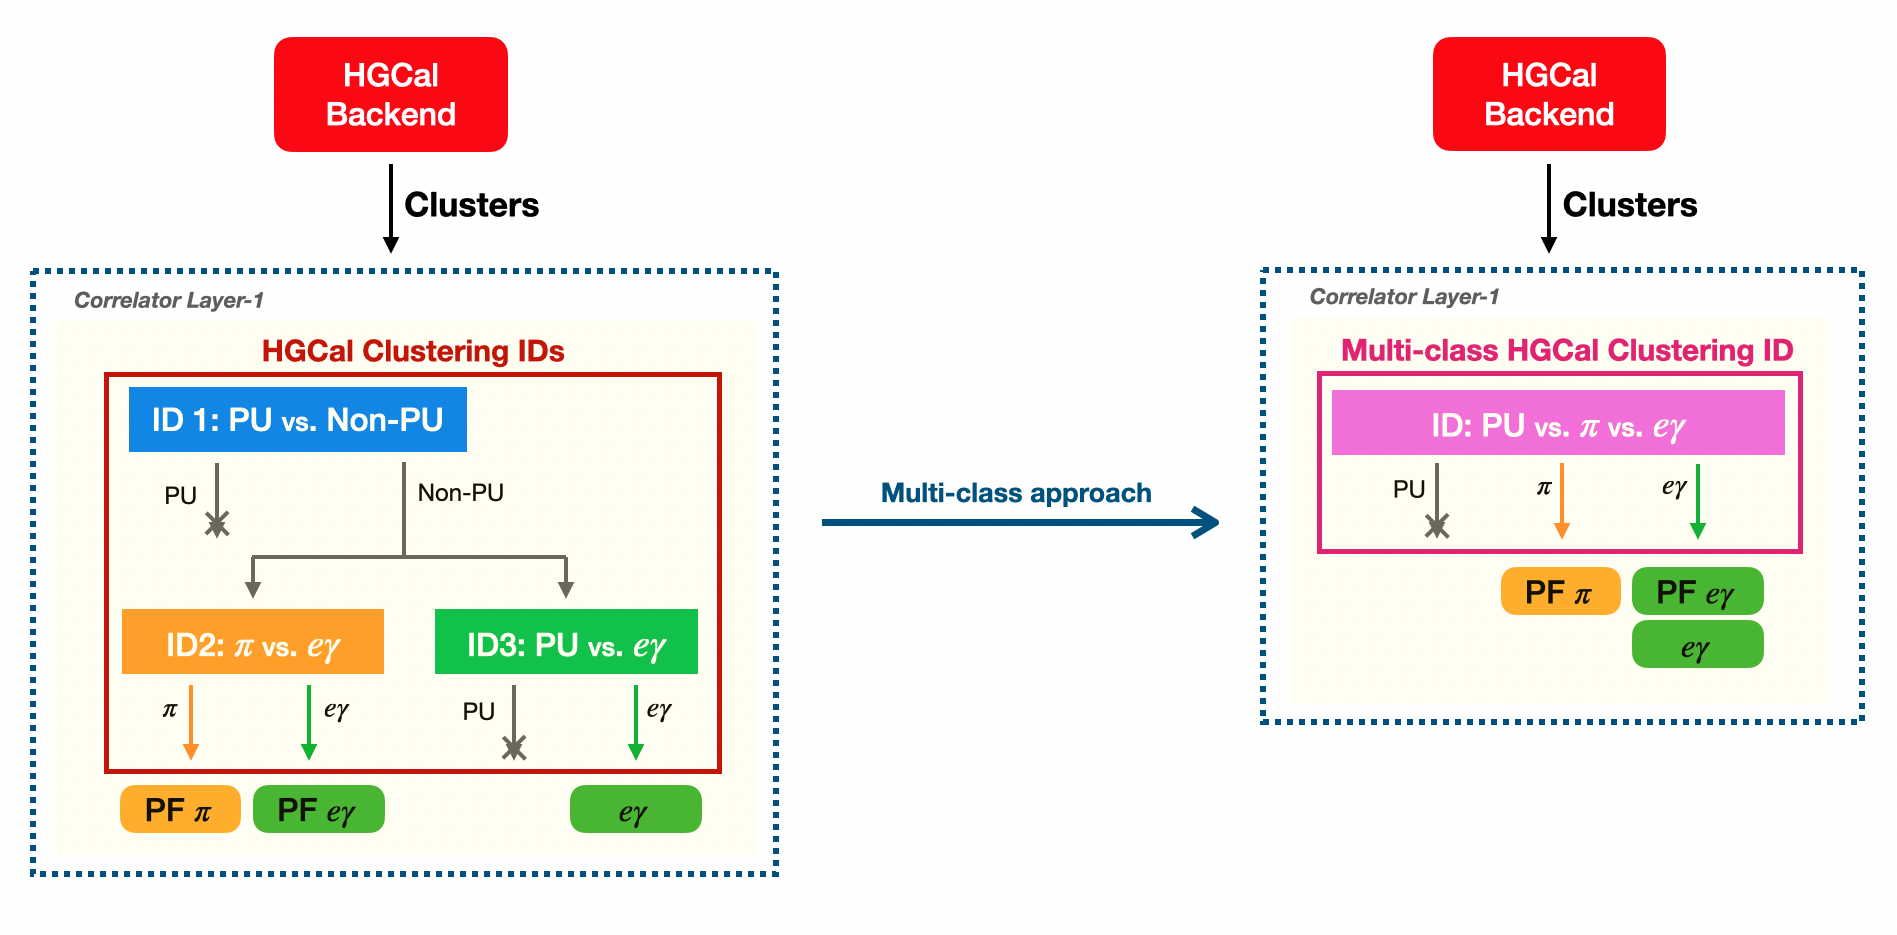
\includegraphics[width=\textwidth]{endcap_figs/HGC_IDschema.png}
\end{figure}

\end{minipage}

\begin{minipage}{\textwidth}
\relscale{0.7}{
The Phase-2 HGCal will cover the pseudorapidity region from 1.52 to 3 with a high transverse and longitudinal granularity. 
HGCal trigger primitives with three-dimensional clustering information will be sent to the L1T Calorimeter and Correlator subsystems. Once the clusters arrive from HGCal backend electronics to the Correlator Trigger, the identification of the clusters takes place in the Correlator Layer-1. The current clustering ID system composed of three separate IDs is shown in the diagram on the left. The clusters that are not identified as pileup (PU) are required to pass two separate IDs for $\pi$ and $e/\gamma$ to build candidates for PF reconstruction and clusters for $e/\gamma$ triggers.
To harmonize and simplify the clustering ID design that is currently in place for Phase-2, a new clustering ID is developed with a multi-class approach using BDT. 
}
\end{minipage}

\end{frame}


\begin{frame}{HGCal Cluster Identification: Multi-class ID}

\begin{columns}[c]

\begin{column}{.5\textwidth}
\begin{figure}
\centering
    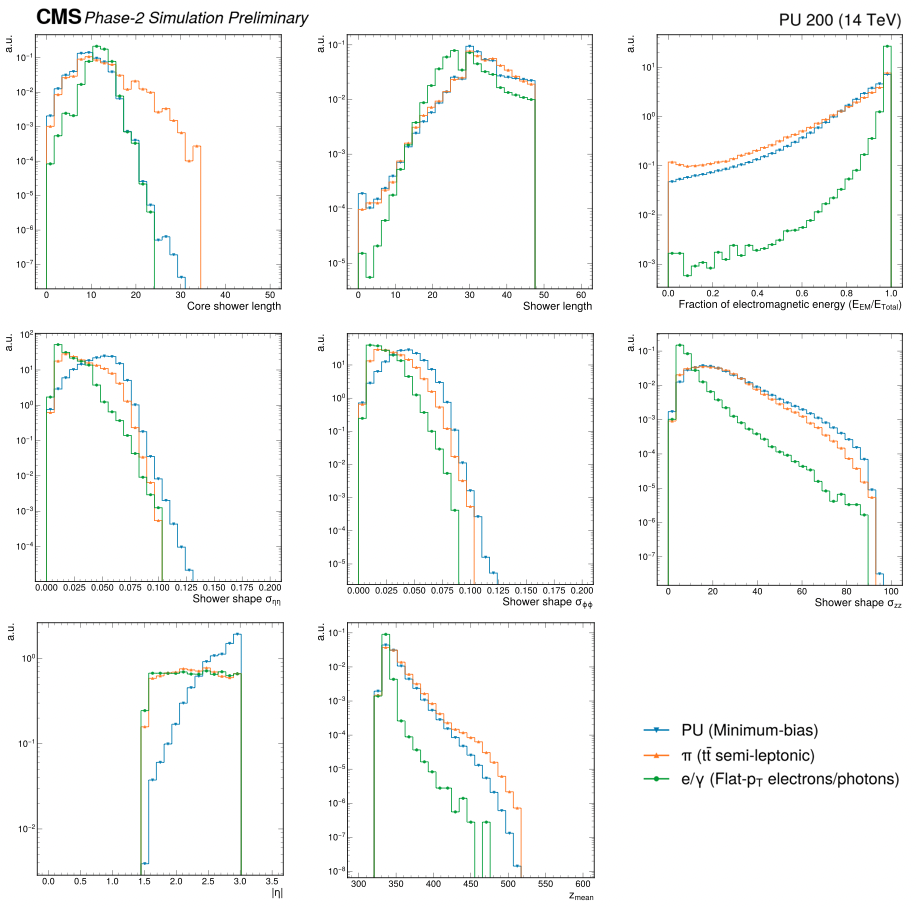
\includegraphics[width=\textwidth]{endcap_figs/HGC_BDTinputs.png}
\end{figure}
\end{column}

\begin{column}{.4\textwidth}
\relscale{0.5}{The plots show the distribution of the input features for building the multi-class BDT ID for each class. These input features based on  HGCal cluster shower kinematics and shapes are used to train an XGBoost~\cite{xgb} BDT model. 
Training datasets are taken from Phase-2 simulation with 200 PU: minimum-bias samples for PU, $t\bar{t}$ semi-leptonic process for $\pi$, and flat $p_{T}$ electron/photon samples for $e/\gamma$, after applying the cut of $p_{T} > 5$ GeV and $\eta < 2.4$ for all clusters and additionally requiring gen-matching of $\Delta R$(gen,~reco)~$< 0.1$ for $\pi$ and $e/\gamma$ clusters. 

Eight cluster features are used as inputs, as shown in the plot from top left to bottom right: core shower length, shower length, fraction of electromagnetic energy $E_{EM}/E_{Total}$, shower shape $\sigma_{\eta\eta}$, $\sigma_{\phi\phi}$,$\sigma_{zz}$, absolute value of cluster pseudorapidity $|\eta|$, and $z_{mean}$.
}
Shower lenghth measures the maximum span of the clusters in terms of the number of HGCal layers. \textit{Core} shower length is the number of continuous shower layers. 
Shower shape $\sigma_{ii} (i=\eta,\phi,z)$ inputs refer to the energy-weighted RMS over cluster constituents. $z_{mean}$ is calculated by the energy-weighted barycenter over the longitudinal coordinate.


\end{column}
\end{columns}

\end{frame}


\begin{frame}{HGCal Cluster Identification: Multi-class ID}


\begin{figure}
\centering
    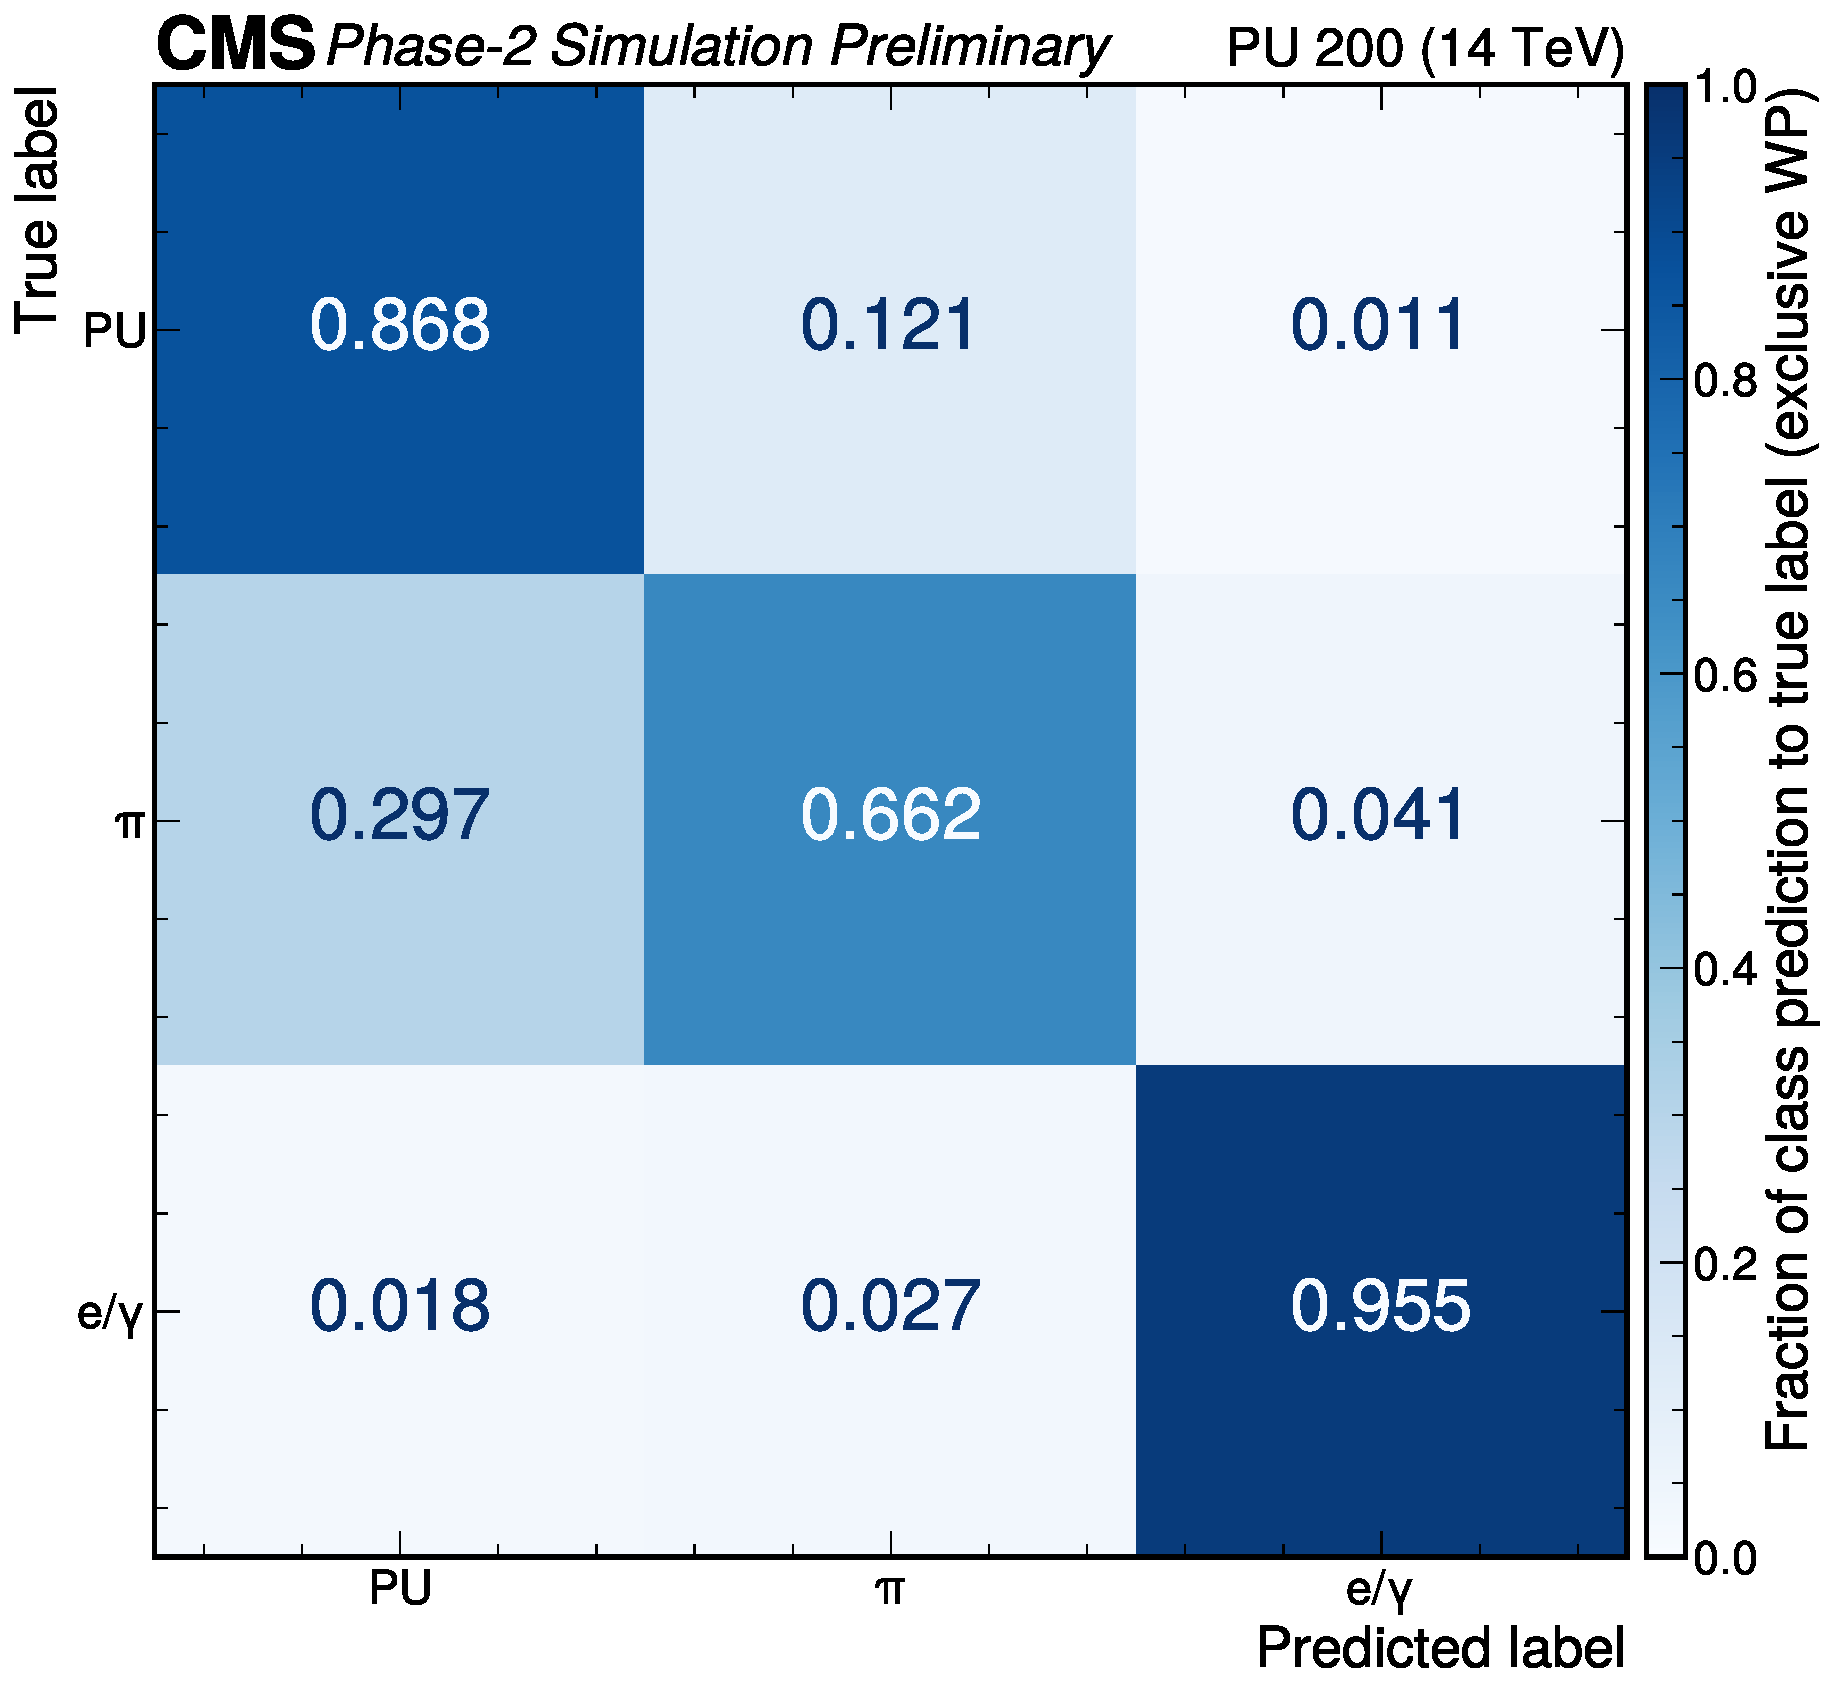
\includegraphics[width=0.27\textwidth]{endcap_figs/HGC_Confusion_Max.pdf}
    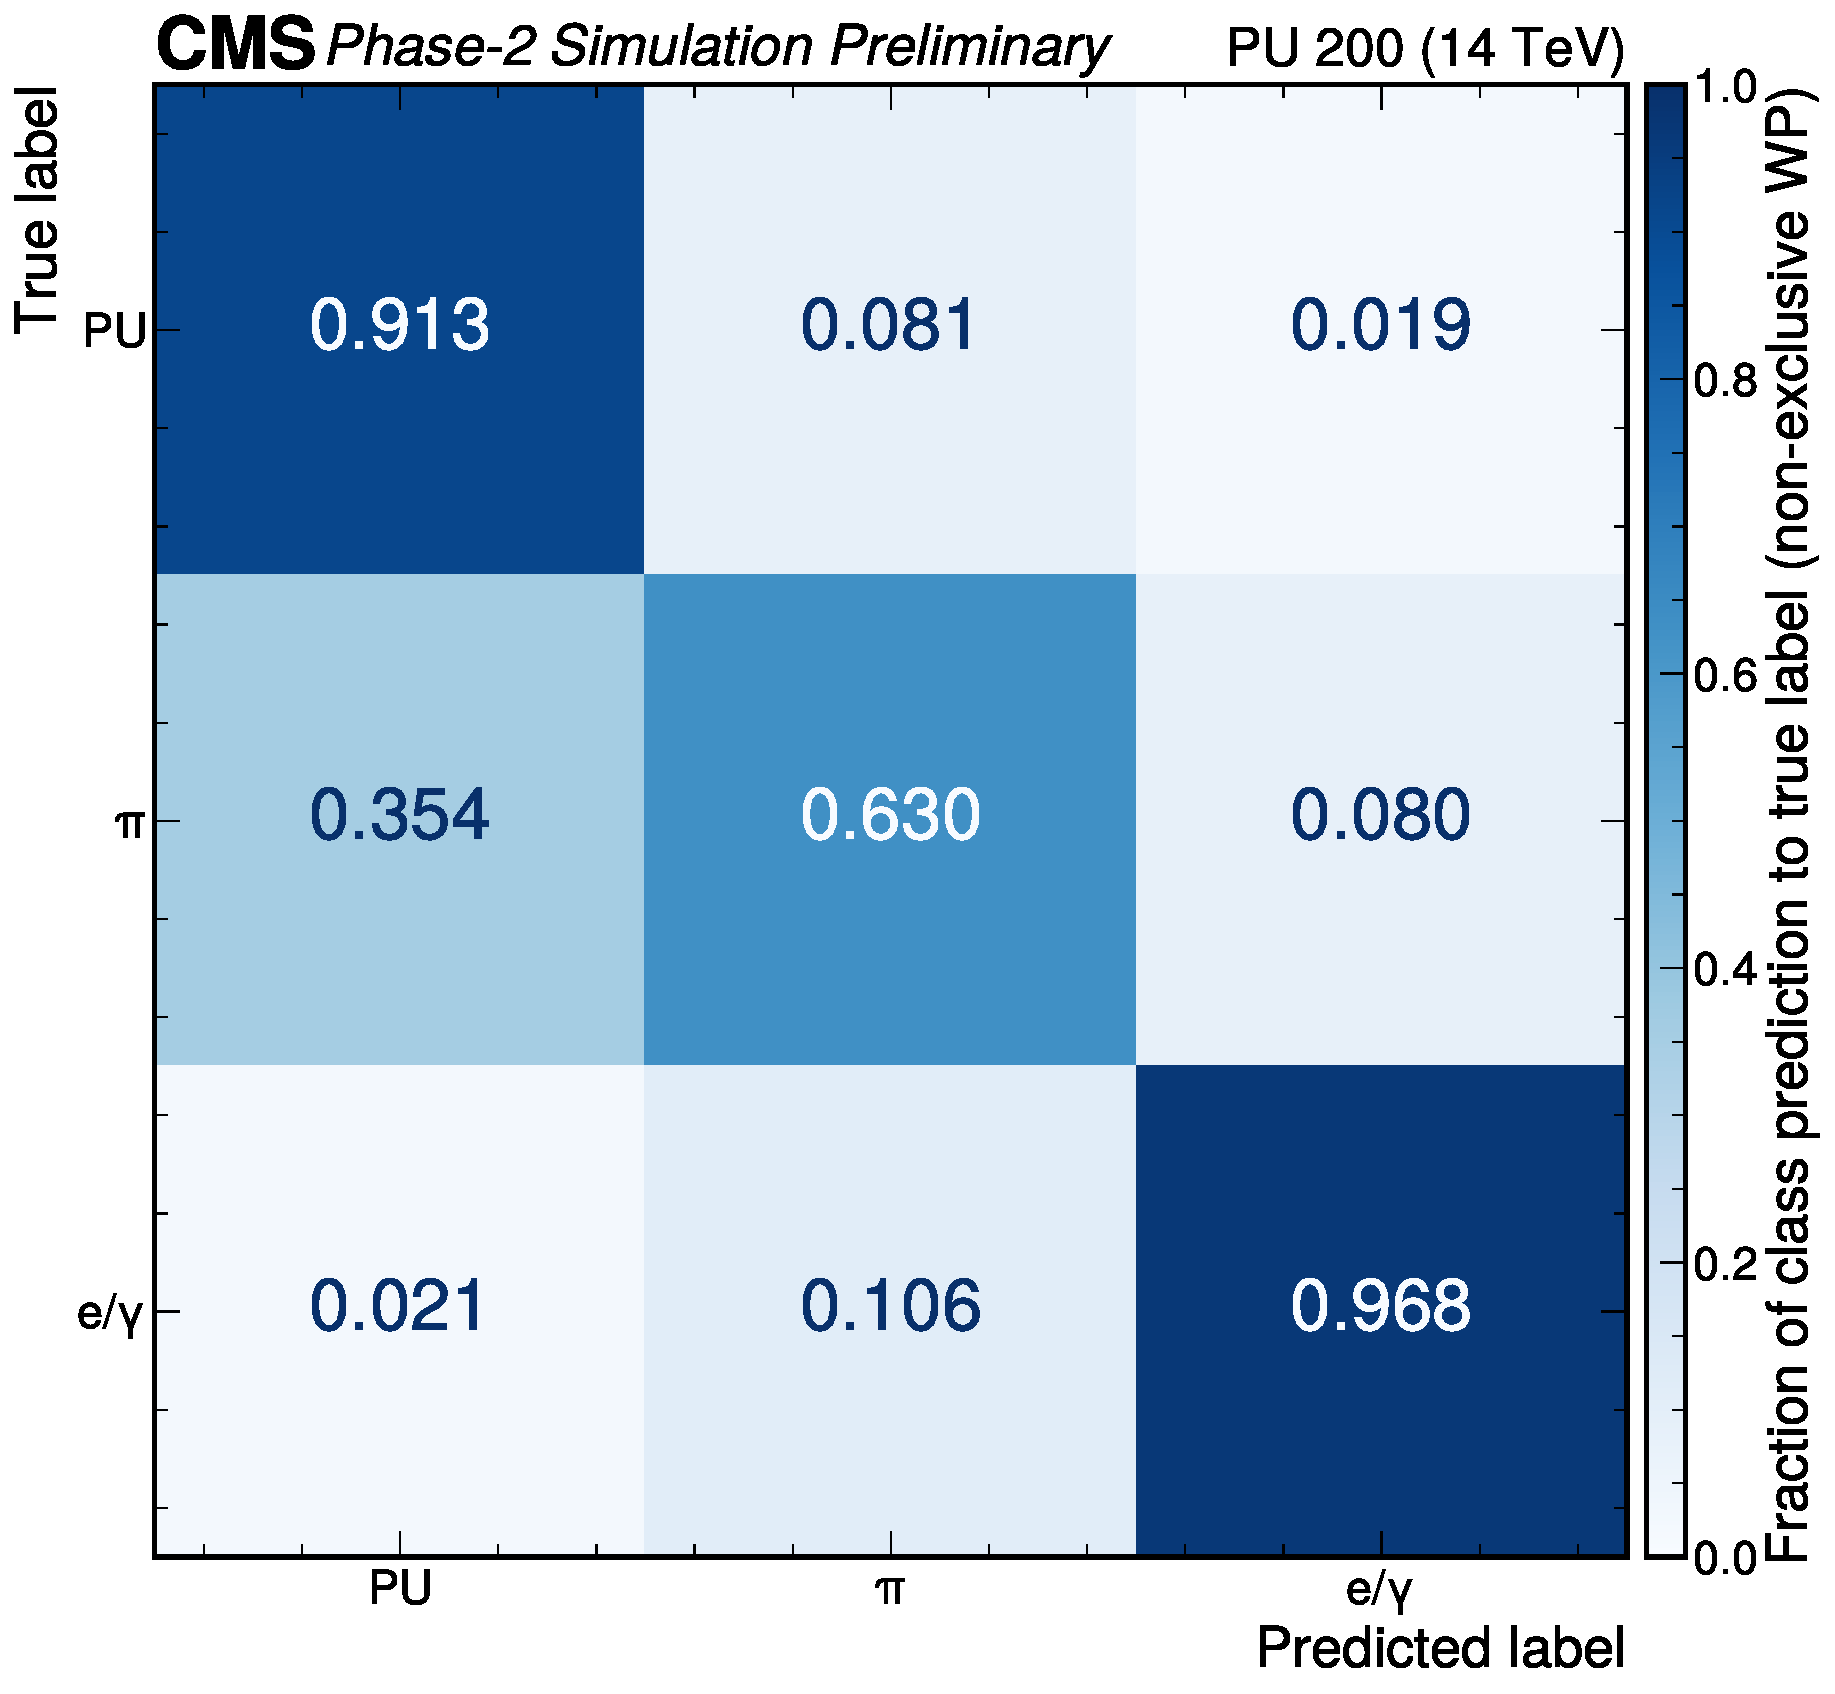
\includegraphics[width=0.27\textwidth]{endcap_figs/HGC_Confusion_Softmax.pdf}
\end{figure}

\begin{minipage}{\textwidth}

\relscale{0.64}{Multi-class BDT for the new clustering ID outputs a vector of BDT scores $\langle \mathrm{PU}, \pi, e/\gamma \rangle$ given a cluster, where the BDT score for each class $i$ represents the probability for the cluster to be of true label $i$. Given the BDT scores, Working Point (WP) is determined by evaluating on Phase-2 simulation with 200 PU: minimum-bias samples for PU, $t\bar{t}$ semi-leptonic process for $\pi$, and flat $p_{T}$ electron/photon samples for $e/\gamma$. Two different schemes for the multi-class ID WP have been studied: \textit{Exclusive WP} and \textit{Non-exclusive WP}. \textit{Exclusive WP} is to identify the cluster as the class with the maximum score from the vector of BDT class outputs. \textit{Non-exclusive WP} is to define a cut on the BDT score for each class, allowing for a cluster to be sometimes identified as more than one class. 

This WP was optimized for the best efficiency and purity of  $e/\gamma$ clusters and to preserve the performance of the PF reconstruction of the MET.

Confusion matrices from using these WP schemes are displayed: \textit{exclusive WP} (left) and \textit{non-exclusive WP} (right). \textit{Non-exclusive WP} scheme is chosen at the end for its better ID efficiency and downstream interpretability.
}

\end{minipage}

\end{frame}


\begin{frame}{HGCal Cluster Identification: Multi-class ID}

\begin{columns}[c]


\begin{column}{.6\textwidth}


\relscale{0.7}{For hardware implementation of the model, the XGBoost model is synthesized via Conifer~\cite{conifer} library with Vitis HLS synthesis tools. The synthesis ran on the Xilinx Virtex UltraScale+ VU13P FPGA with a clock cycle of 2.78\,ns. Floating value input features are quantized to ap\_fixed~$\langle 20,10 \rangle$, corresponding to seven bits for the integer and ten bits for the decimal. The tables show the latency and FPGA resources used by the new multi-class clustering ID \textcolor{blue}{in terms of the used fraction of Block Random Access Memory (BRAM), Digital Signal Processors (DSPs), flip-flops (FF), and lookup tables (LUTs), both in the Super Logic Region (SLR) and the whole FPGA.}

The plot shows the ID efficiency for each class as a function of $p_{T}$, comparing between XGBoost BDT model with floating inputs and the synthesized model with quantized inputs. The evaluation of the ID efficiency is done on Phase-2 simulation with 200 PU: minimum-bias samples for PU, $t\bar{t}$ semi-leptonic process for $\pi$, and flat $p_{T}$ electron/photon samples for $e/\gamma$ clusters. 

}
\end{column}

\begin{column}{.4\textwidth}

\resizebox{\textwidth}{!}
{
\begin{tabular}{rccccc}
\hline
  & BRAM & DSP & FF & LUT \\
\hline
SLR & 0.0\%& 0.0\% & 1.0\% & 25.0\% \\
Total & 0.0\%& 0.0\% & 0.0\% & 6.0\% \\
\hline
\end{tabular}
}

\begin{table}
\resizebox{\columnwidth}{!}{%
\begin{tabular}{ccc}
\hline
& Latency (cycles) & Latency (absolute) \\
\hline
Clock (2.78\,ns) & 5 & 13.890\,ns \\
\hline
\end{tabular}
}
\end{table}

\begin{figure}
\centering
    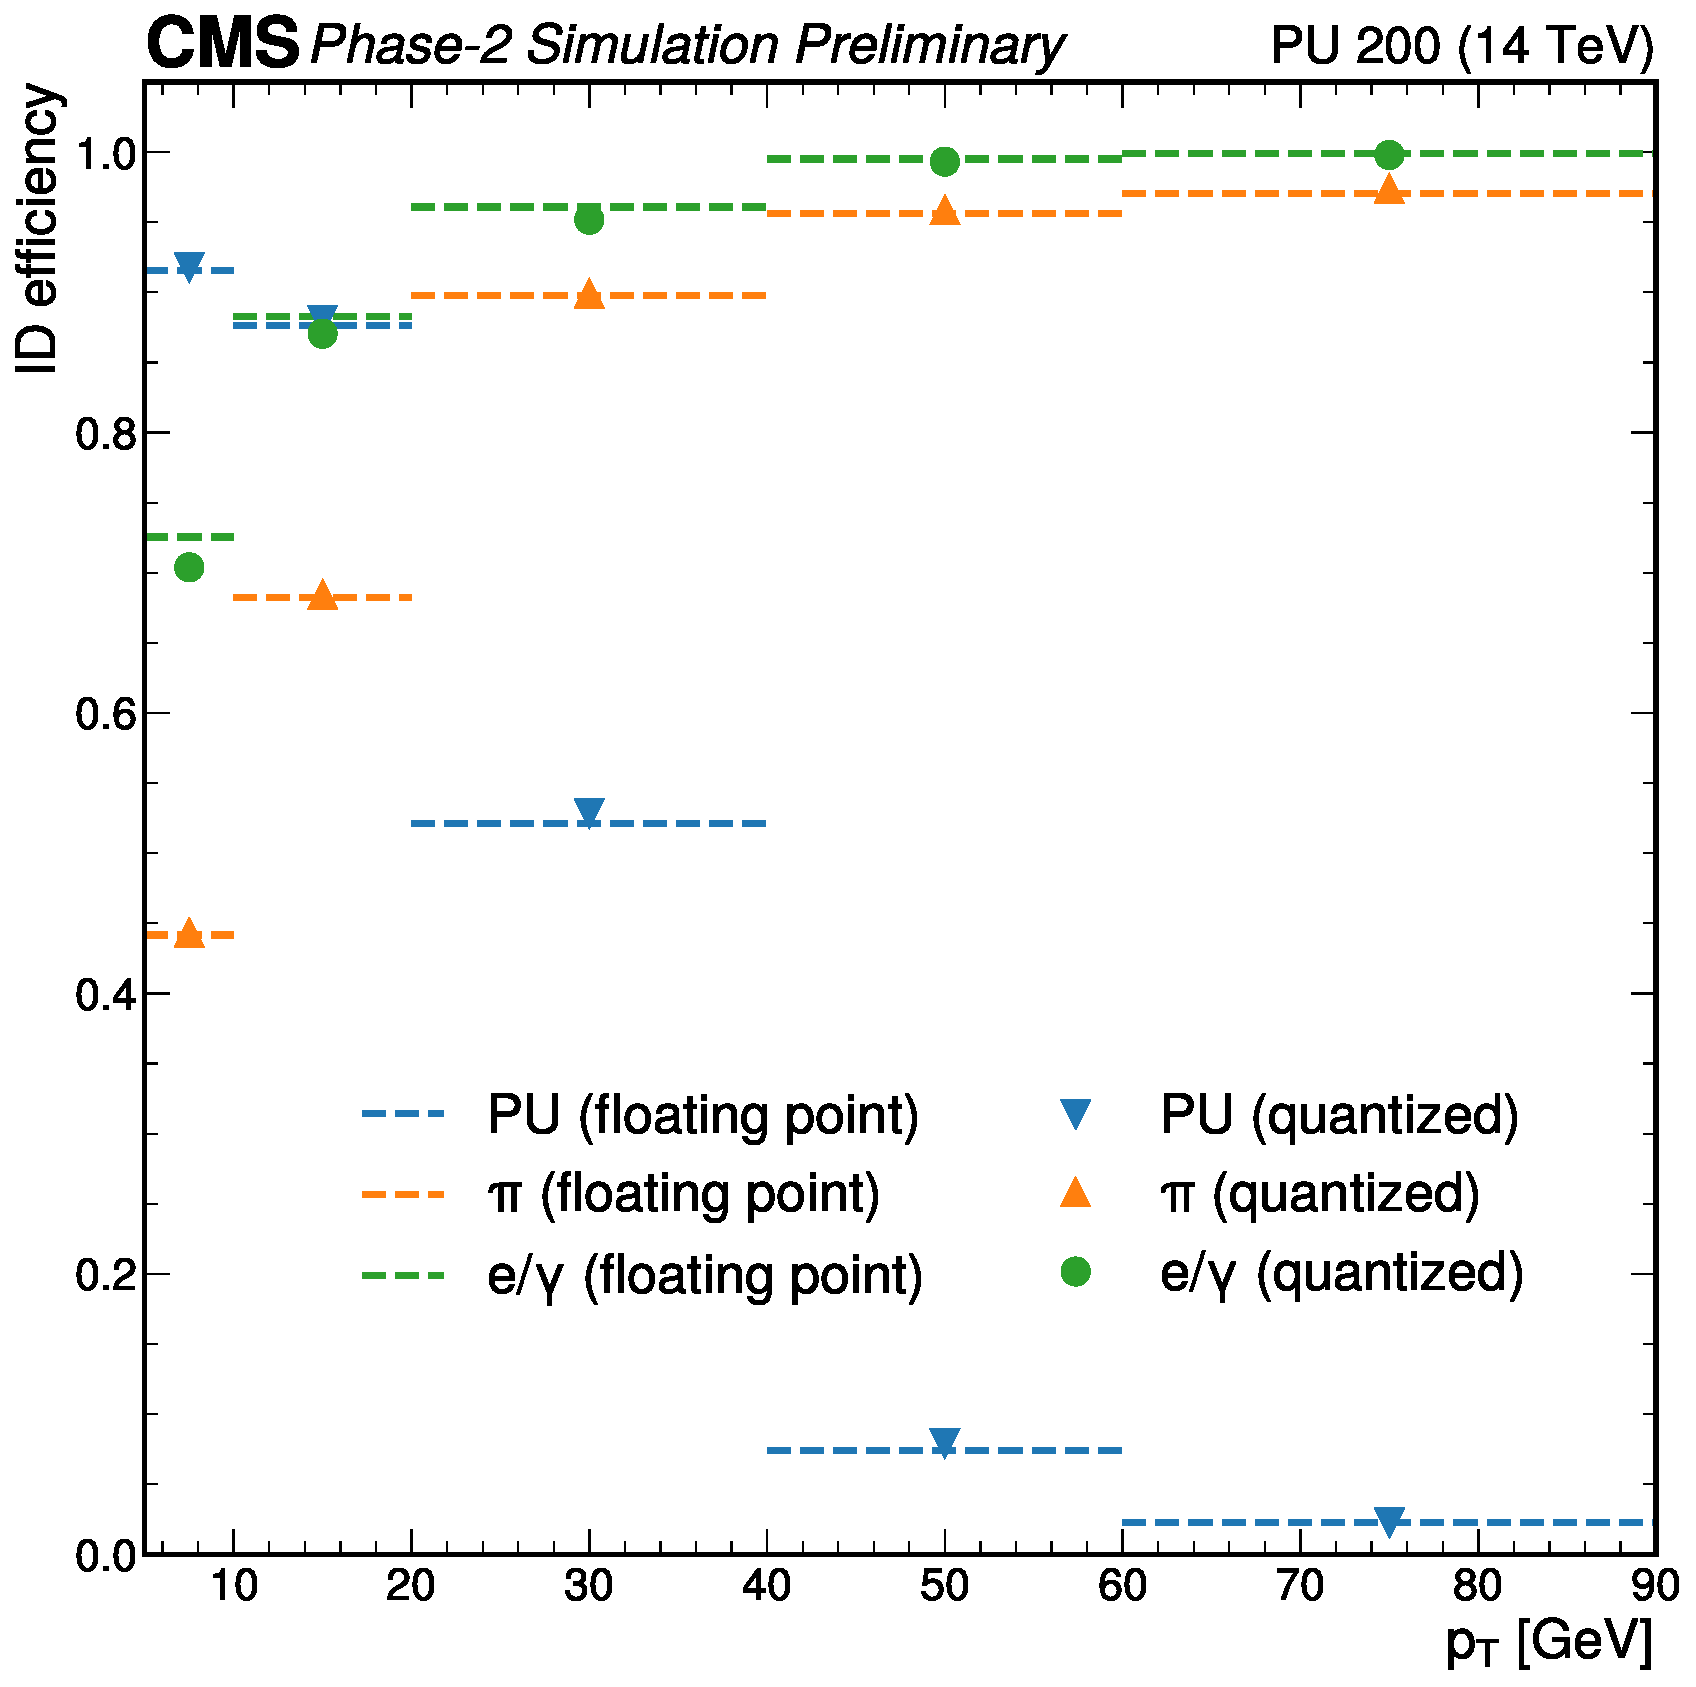
\includegraphics[width=0.7\textwidth]{endcap_figs/HGC_eff_xgb_conifer.pdf}
\end{figure}


\end{column}


\end{columns}

\end{frame}


\begin{frame}{HGCal Cluster Identification: Multi-class ID}

\begin{figure}
\centering
    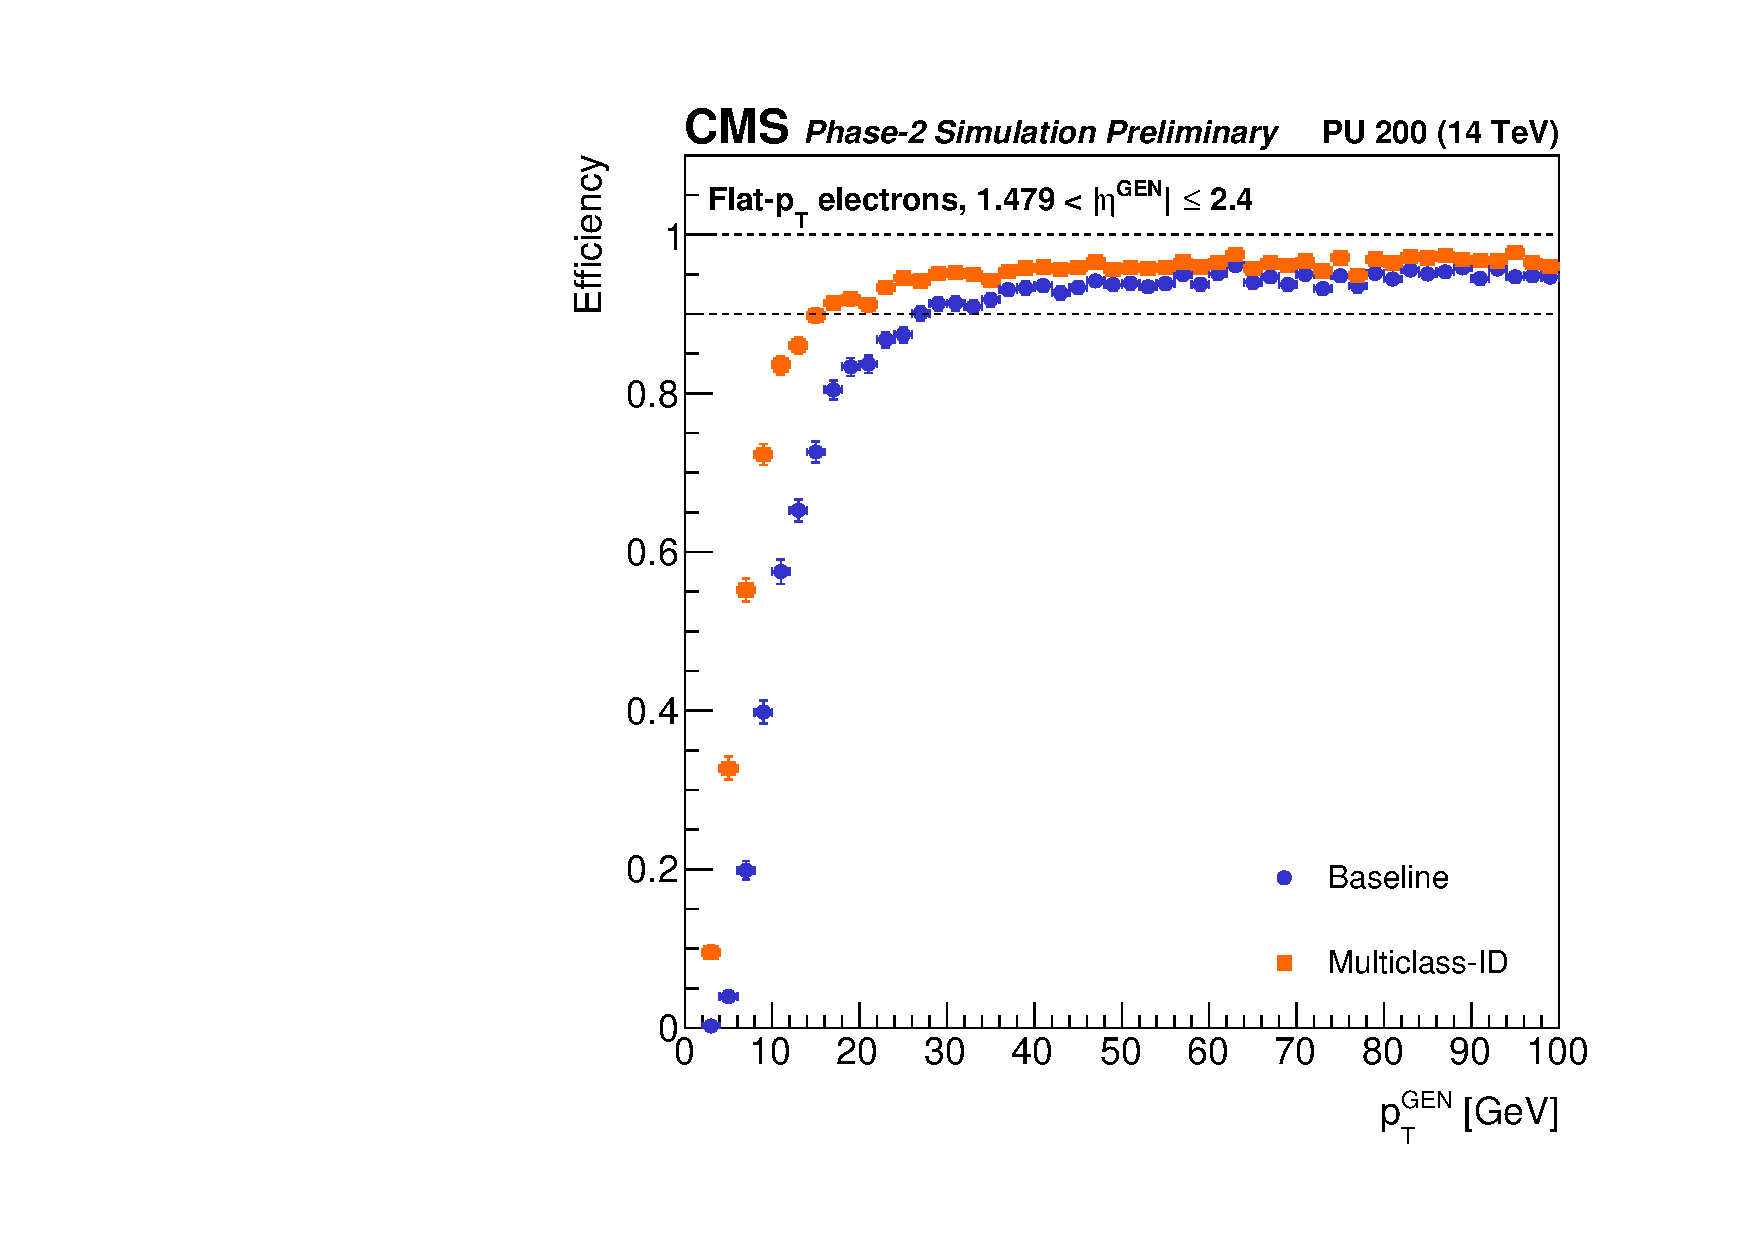
\includegraphics[width=0.31\textwidth]{endcap_figs/HGC_EgEff_Pt.pdf}
    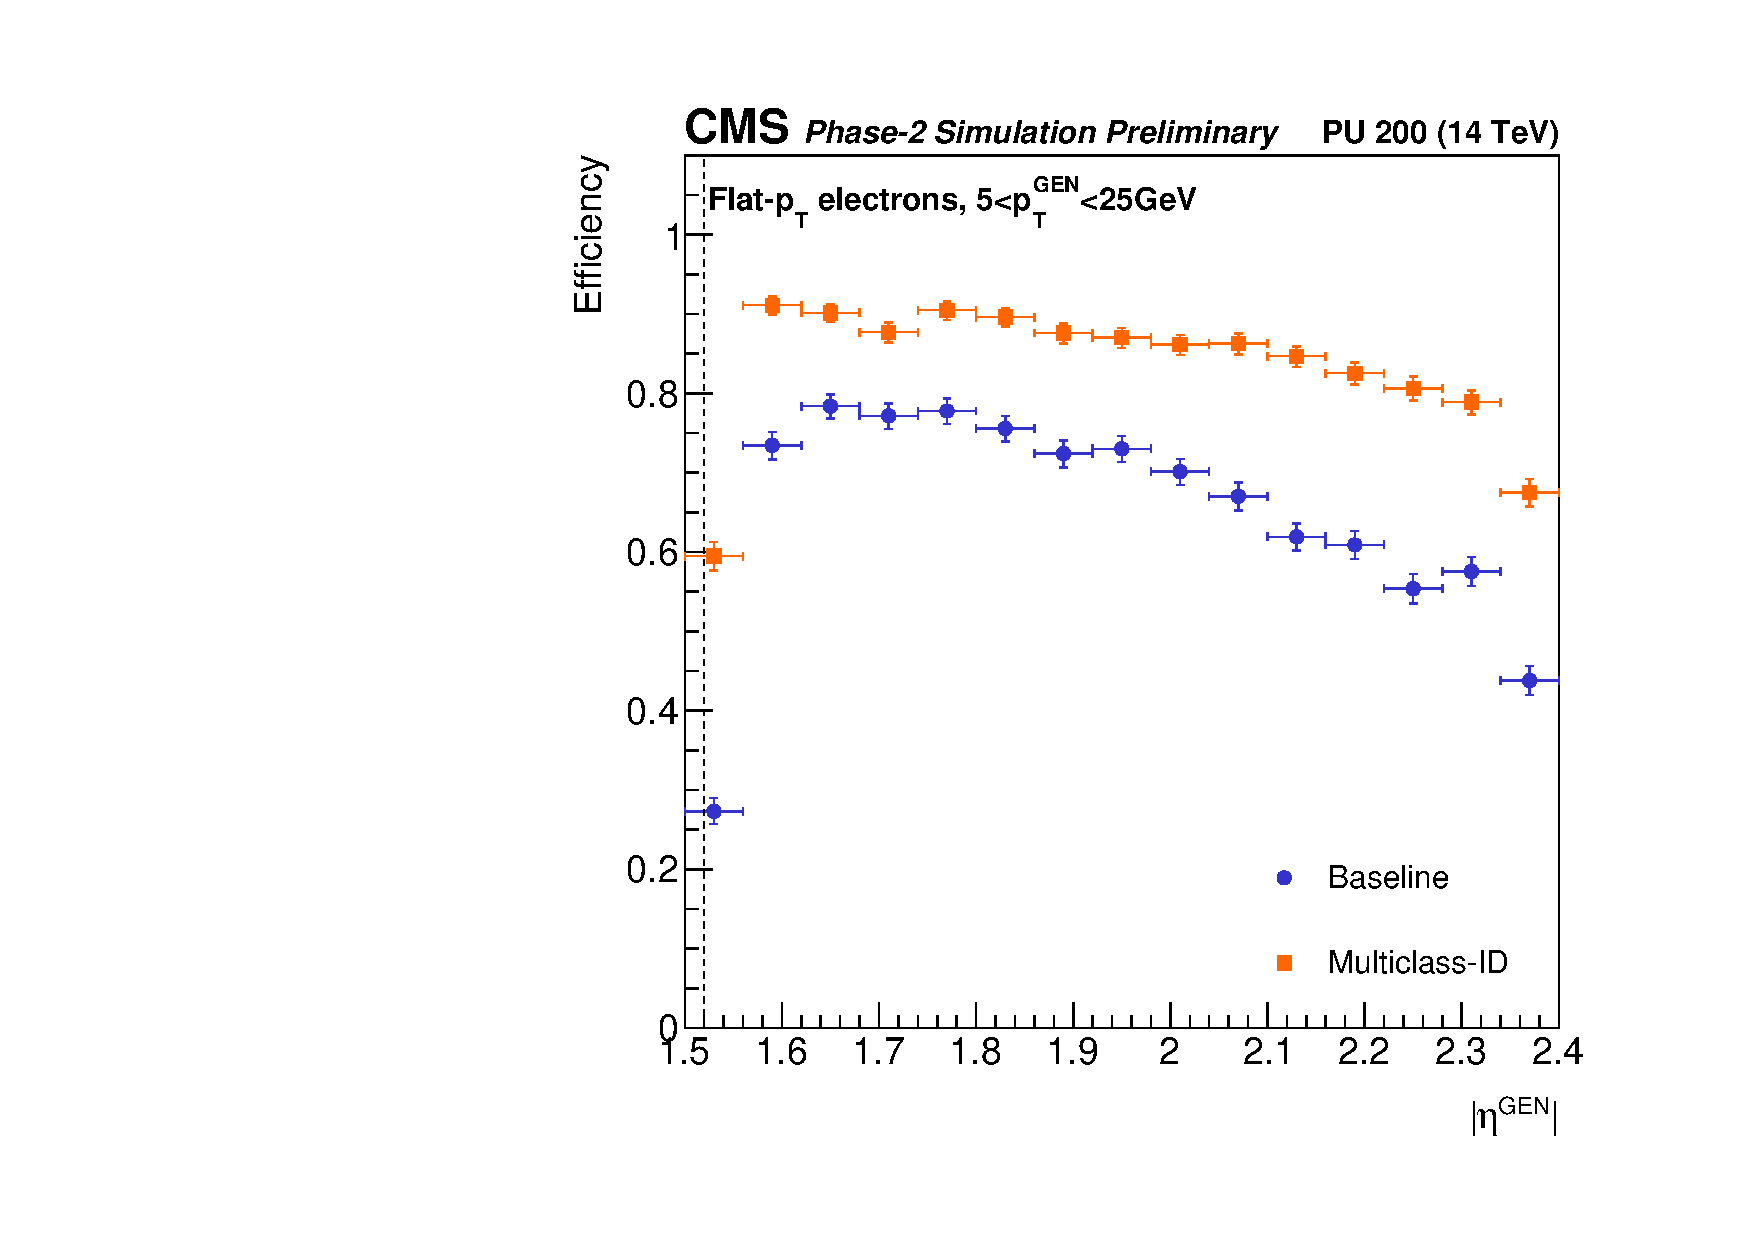
\includegraphics[width=0.31\textwidth]{endcap_figs/HGC_EgEff_EtaPt5to25.pdf}
    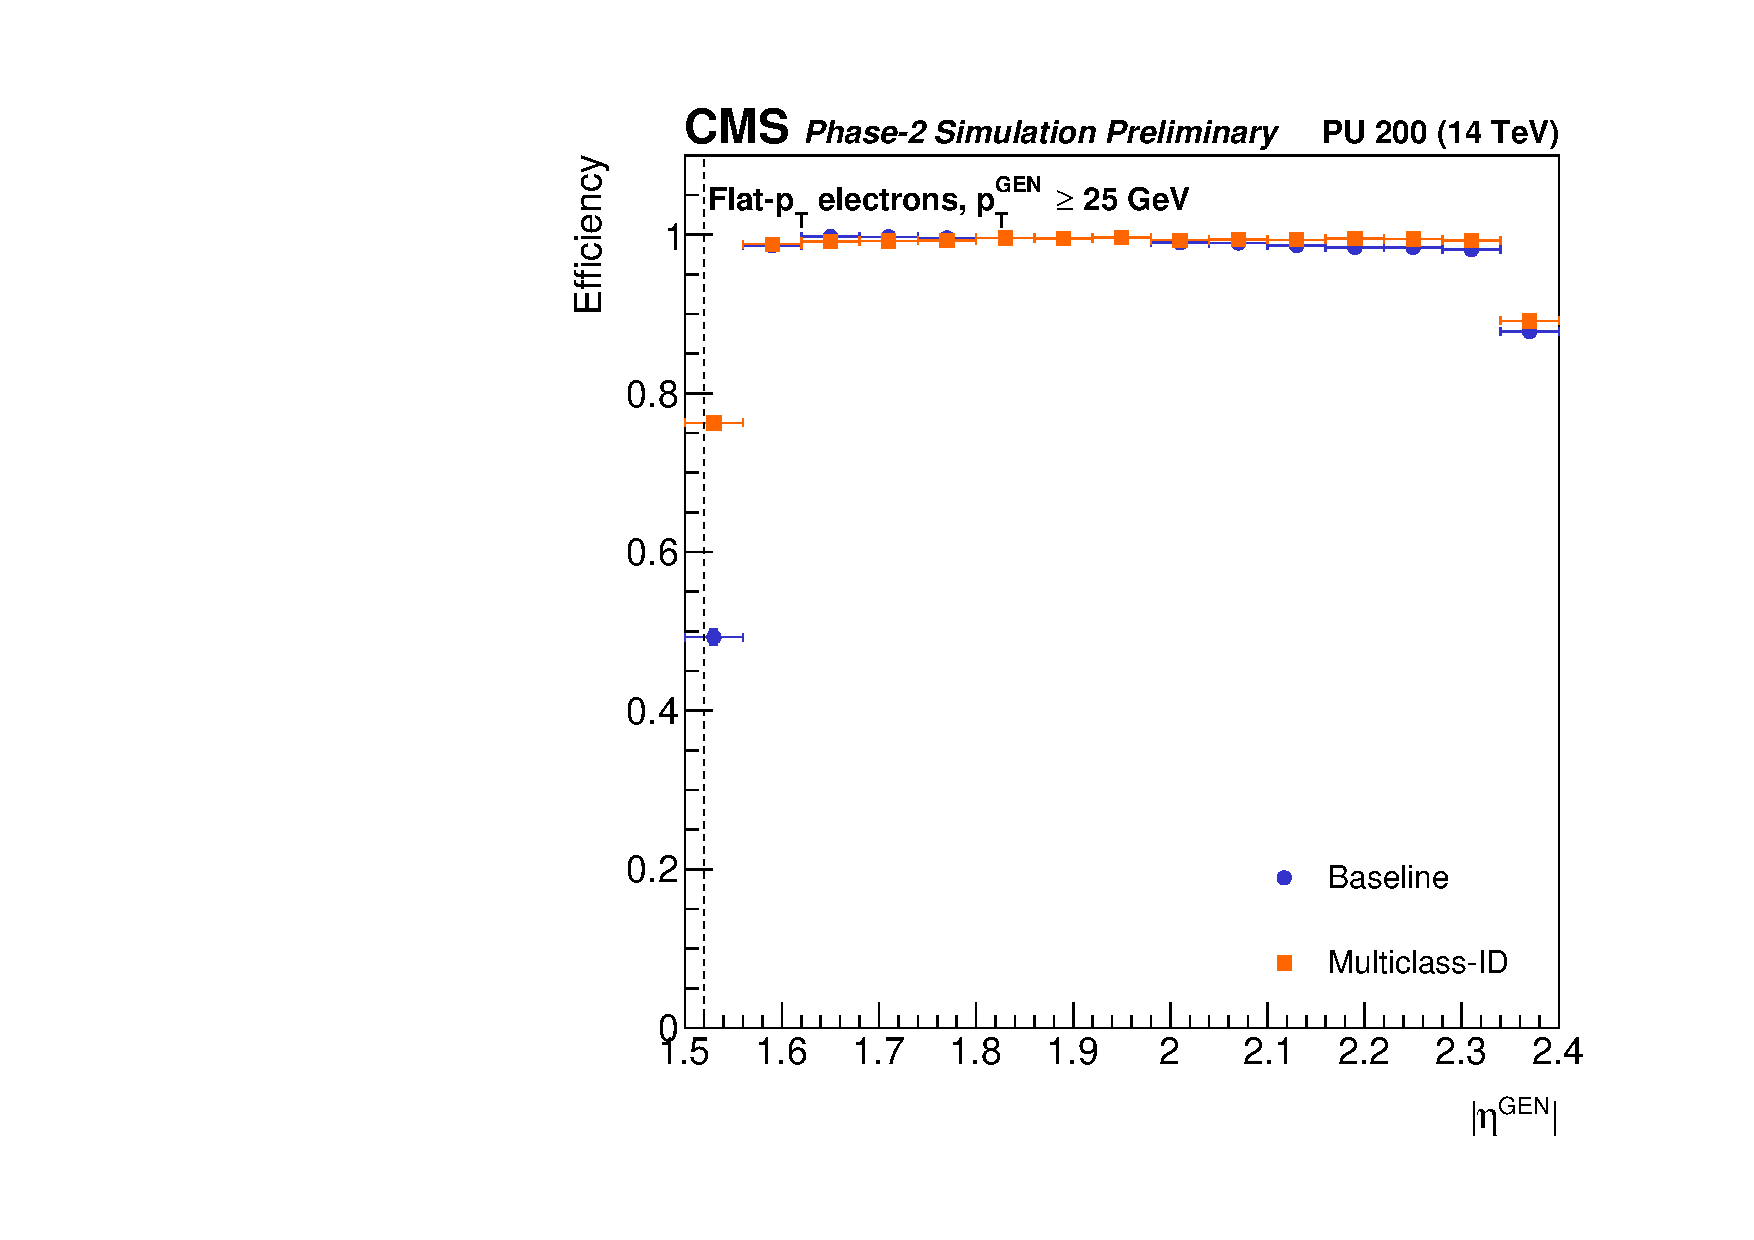
\includegraphics[width=0.31\textwidth]{endcap_figs/HGC_EgEff_EtaPt25.pdf}
\end{figure}


\begin{minipage}{\textwidth}
\relscale{0.666}{The plots compare the efficiency of reconstructing a genuine electron at L1T for the baseline and the new multiclass $e/\gamma$ IDs for standalone electromagnetic objects on a flat-$p_{T}$ electron sample. The efficiency as a function of the generator-level $p_{T}$ (left) and pseudorapidity (middle and right) is illustrated. \textcolor{blue}{In the central and right plots, the vertical dashed line represents the transition region between the barrel and the endcaps.} The efficiency at the low $p_{T}$ region is significantly improved with the new multi-class ID, e.g. an overall 35\% improvement in efficiency for $5 < p_{T} < 10$\,GeV. 
The efficiency improves throughout the whole endcap $\eta$ coverage.
While only high-$p_{T}$ standalone electromagnetic objects ($p_{T} > 25$\,GeV) are used in the TDR Trigger Menu~\cite{tdr-p2-l1}, efficient identification of 
low-$p_{T}$ clusters can be exploited in building track-matched electrons and in the L1T Scouting system to target signals with low-$p_{T}$ electrons.
}

\end{minipage}

\end{frame}



\begin{frame}{HGCal Cluster Identification: Multi-class ID}

\begin{figure}
\centering
    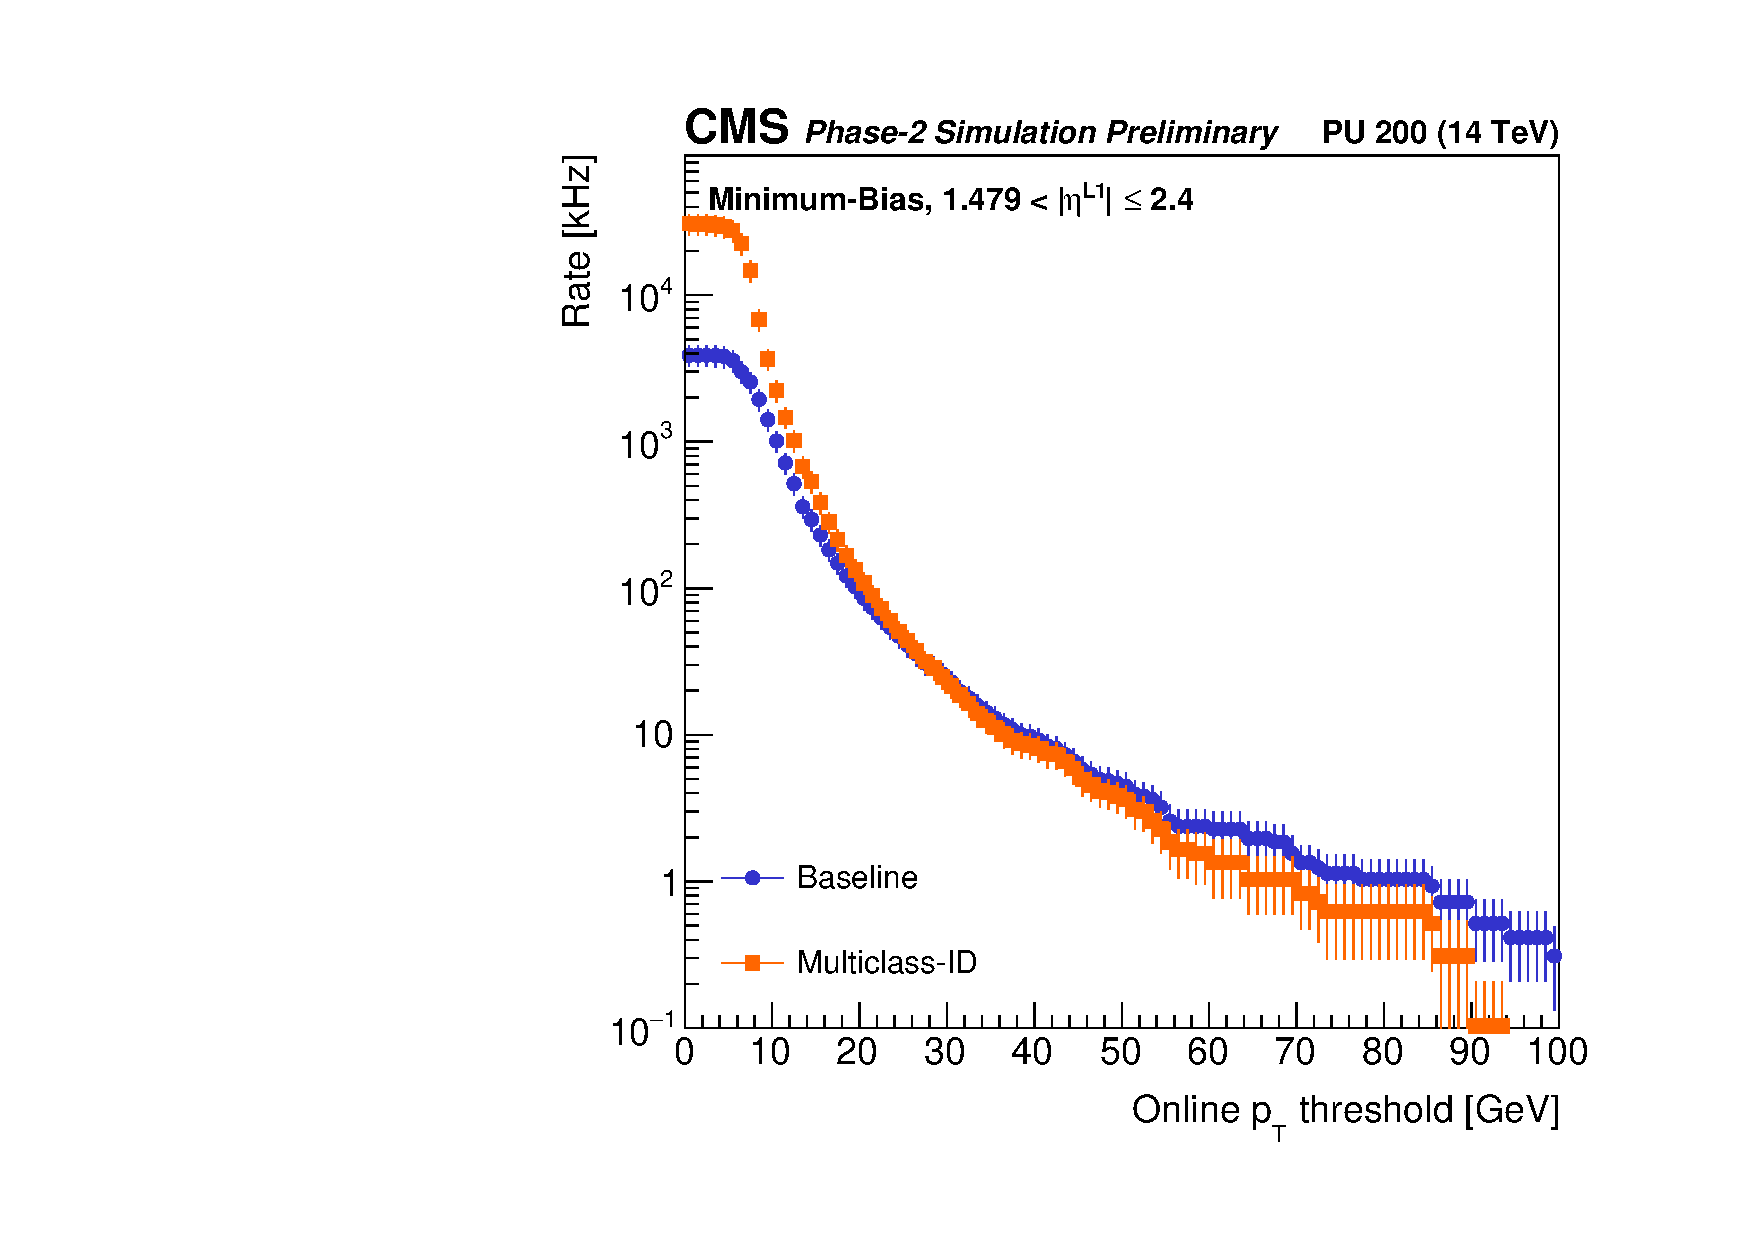
\includegraphics[width=0.35\textwidth]{endcap_figs/HGC_Rate_TkEmEE.pdf}

\end{figure}



\begin{minipage}{\textwidth}
\relscale{0.7}{The plot shows the rates of standalone electromagnetic objects measured on minimum bias samples, comparing the current baseline and new multi-class clustering ID. The multi-class ID increases the rate in low $p_{T}$ regions but lowers it at the typical thresholds used in the TDR baseline Trigger Menu ($p_{T} > 25$\,GeV).}
\end{minipage}

\end{frame}












\section{Electrons in the Phase-2 Level-1 Trigger in the ECAL barrel region}


\begin{frame}{Electrons in the Phase-2 Level-1 Trigger in the ECAL barrel region}
\begin{figure}
\centering
    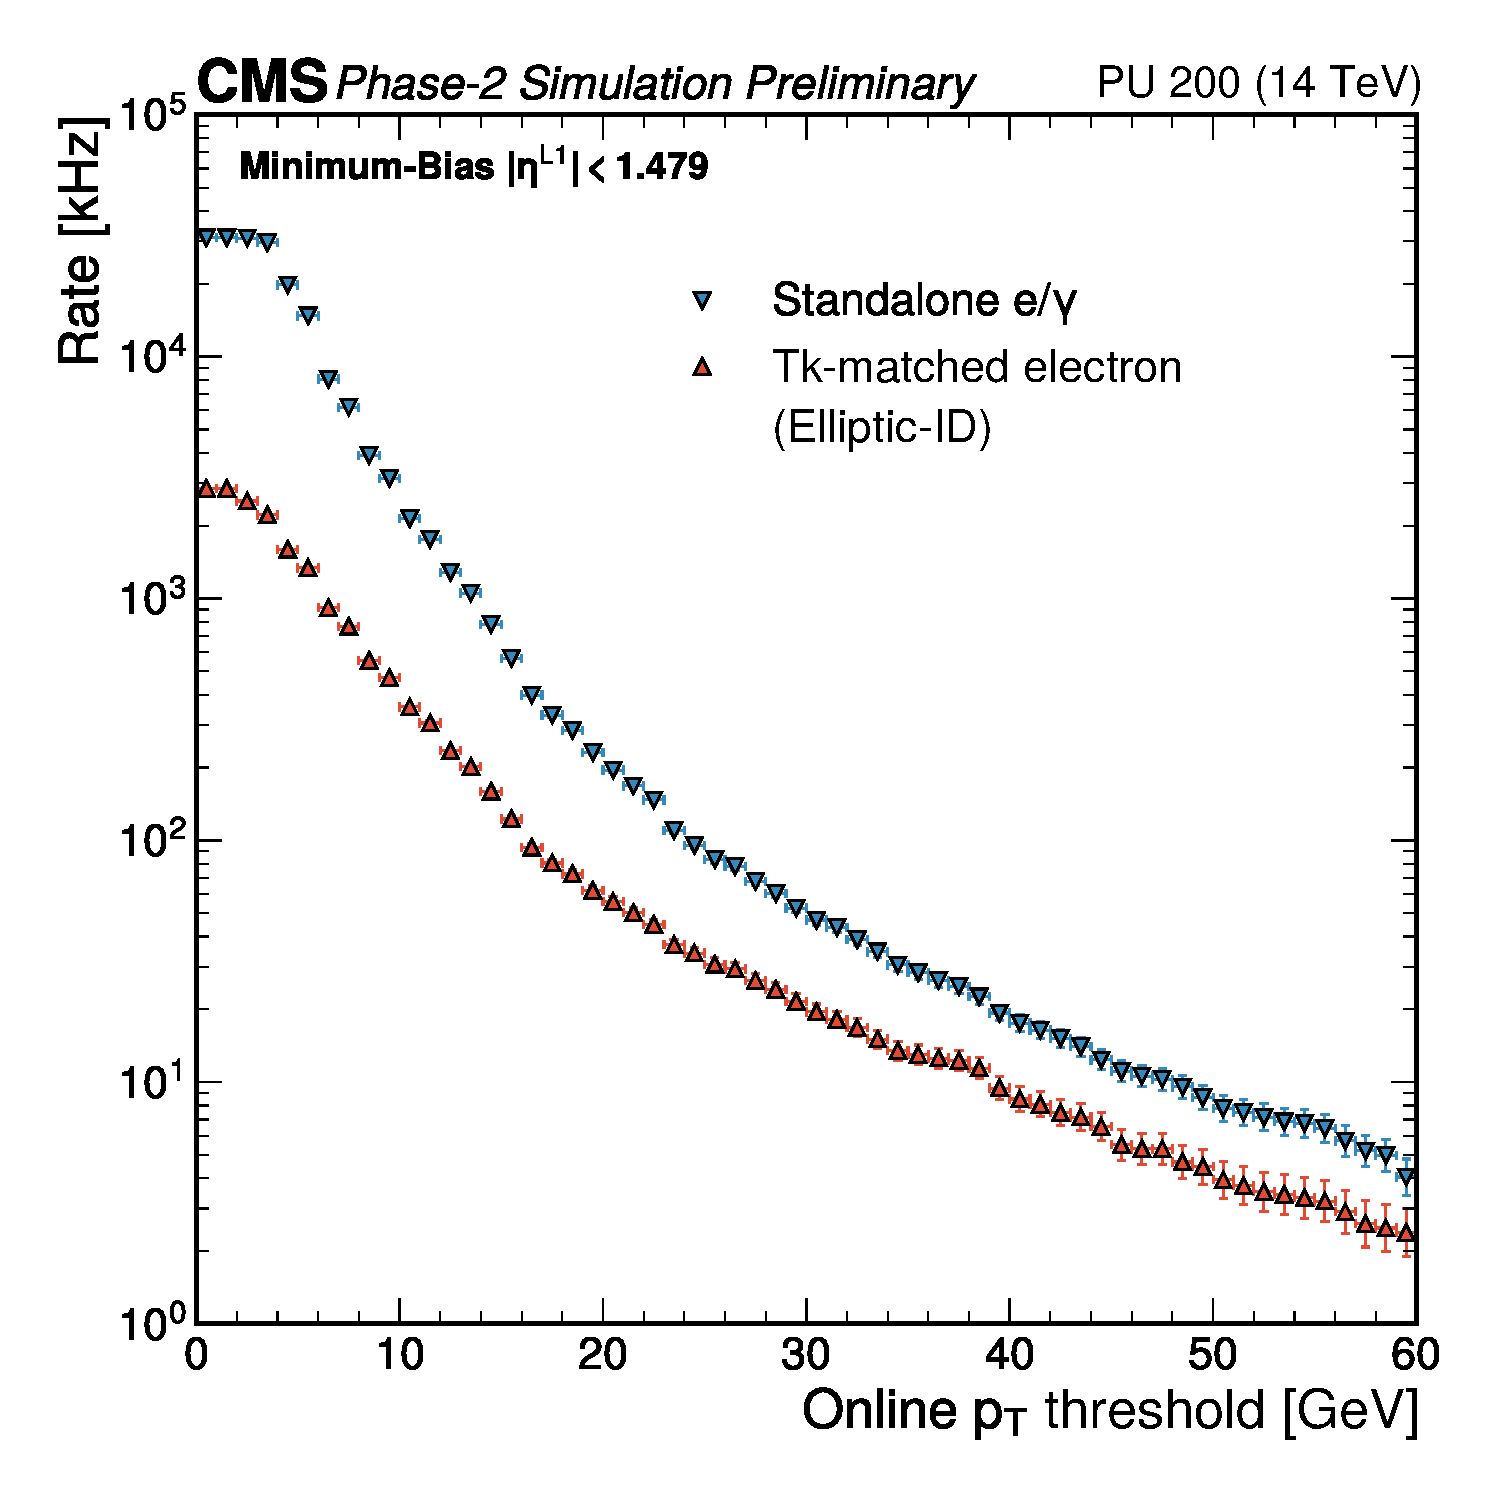
\includegraphics[width=0.4\textwidth]{barrel_figs/slides15/rate.pdf}
    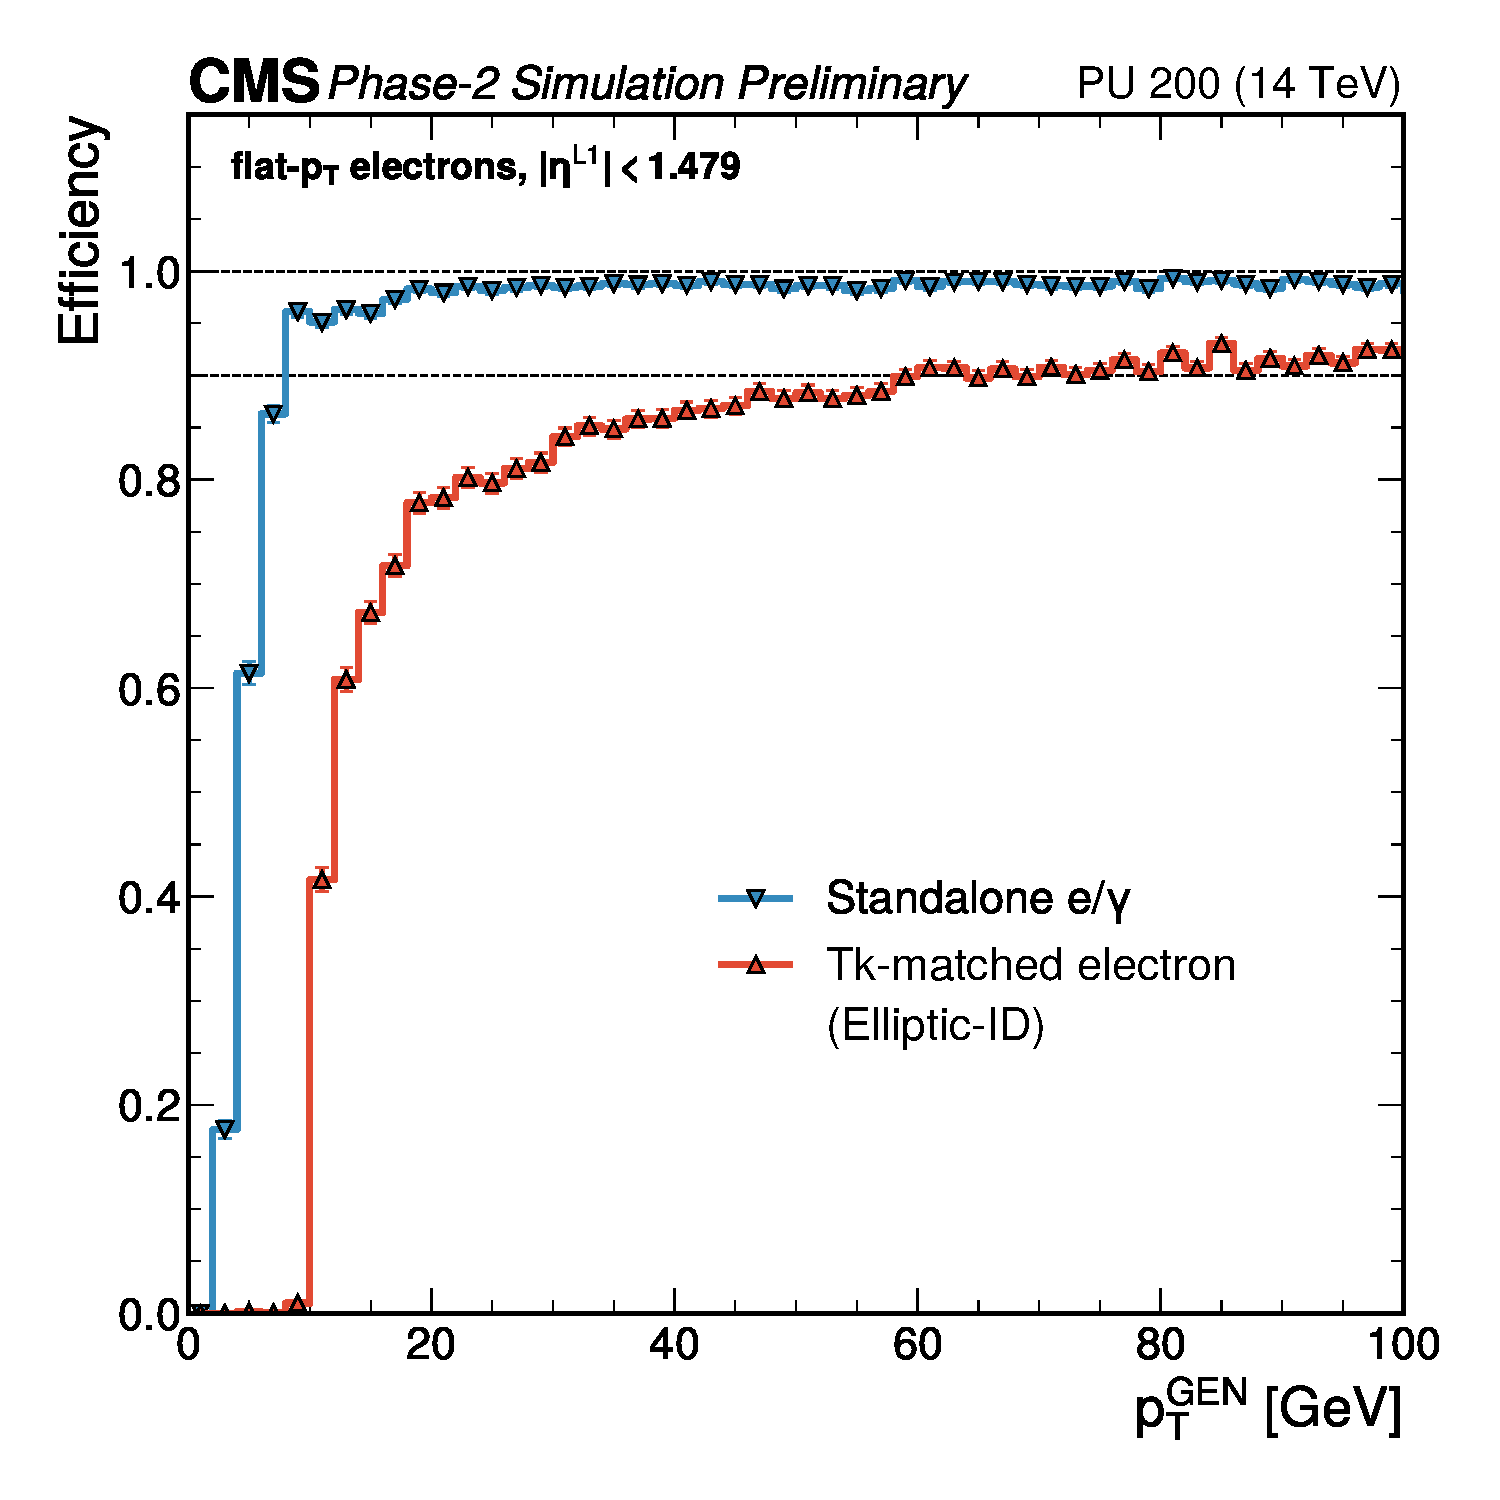
\includegraphics[width=0.4\textwidth]{barrel_figs/slides15/pteff.pdf}

\end{figure}



\begin{minipage}{\textwidth}
\relscale{0.635}{
Matching calorimeter deposits to tracks for identifying electrons is pivotal for sustaining the typical Single and Double Electron trigger thresholds of the TDR Menu. The plot on the left illustrates the comparison between the rate of events on a Minimum Bias sample with an average of 200 pileup when requiring a standalone calorimeter object or a track-matched object at different $p_{T}$ thresholds.
The right plot shows the trigger efficiency as a function of the transverse momentum of the generated electron for the same objects.
The efficiency plots are obtained on a flat-$p_{T}$ electron sample using the TDR baseline matching algorithm called \emph{Elliptic-ID} \cite{tdr-p2-l1}.}
\end{minipage}

\end{frame}



\section{Electron Reconstruction and Identification in the barrel: Composite ID}

\begin{frame}{Track-matched Electron Identification in the barrel}

\begin{columns}[c]

\begin{column}{.7\textwidth}
\begin{minipage}{\textwidth}
The baseline identification technique (\emph{Elliptic-ID}) relies on the independent selection of electromagnetic calorimeter clusters and L1 tracks followed by an angular matching procedure~\cite{tdr-p2-l1}. Electrons' track quality and momentum resolution often suffer because of distortions due to bremsstrahlung radiation. A minimum $p_{T}$ cut of \unit[10]{GeV} is applied to the track to control the combinatorics and the rate.
\\
A new machine learning approach called \emph{Composite-ID}, combines information about tracks and clusters in the barrel into a single model for matching and identification.
\end{minipage}
\end{column}


\begin{column}{.35\textwidth}
\begin{figure}
\centering
    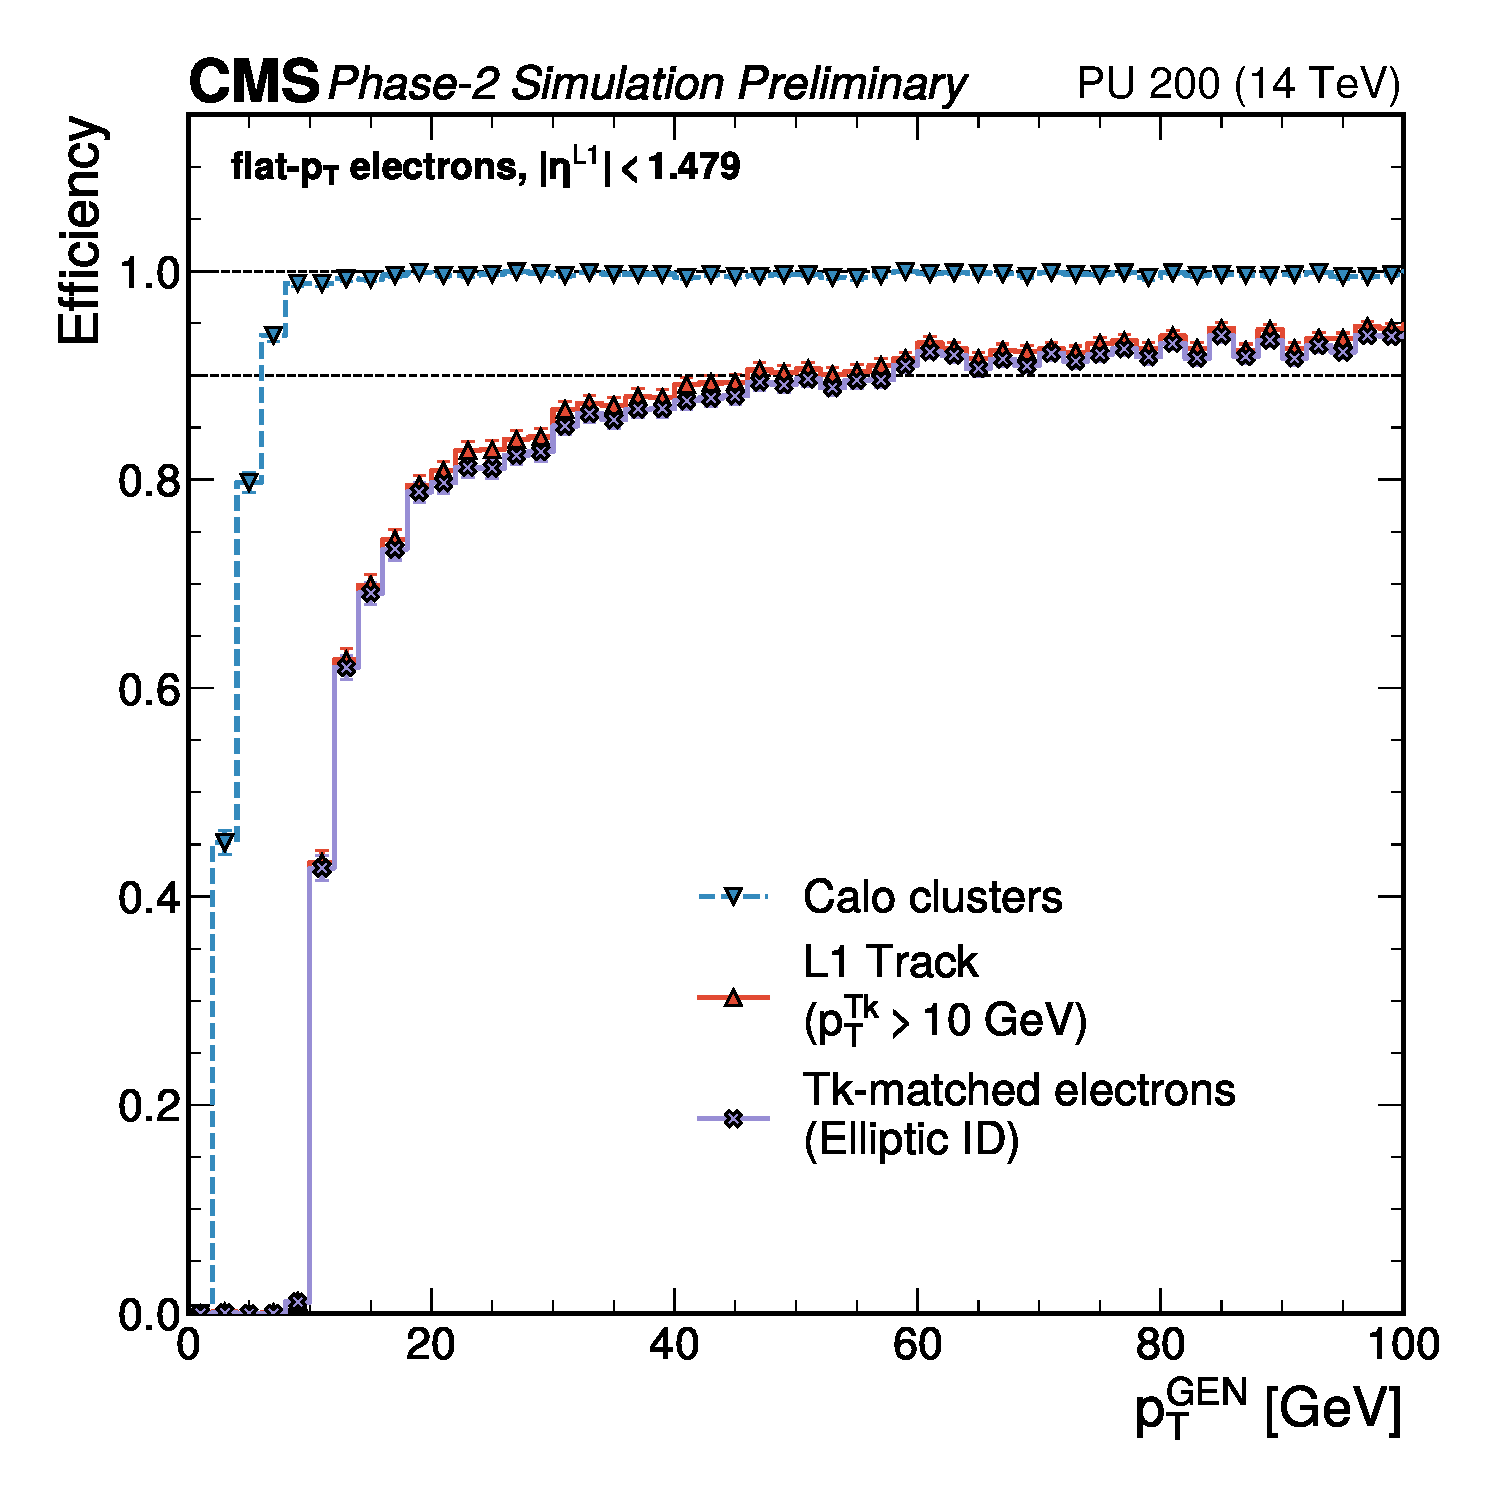
\includegraphics[width=\textwidth]{barrel_figs/slides16/pteff.pdf}
\end{figure}
\end{column}

\end{columns}
\end{frame}



\begin{frame}{Tk-matched Electrons in the barrel: Composite-ID Candidates}

    

    


\begin{figure}
\centering
    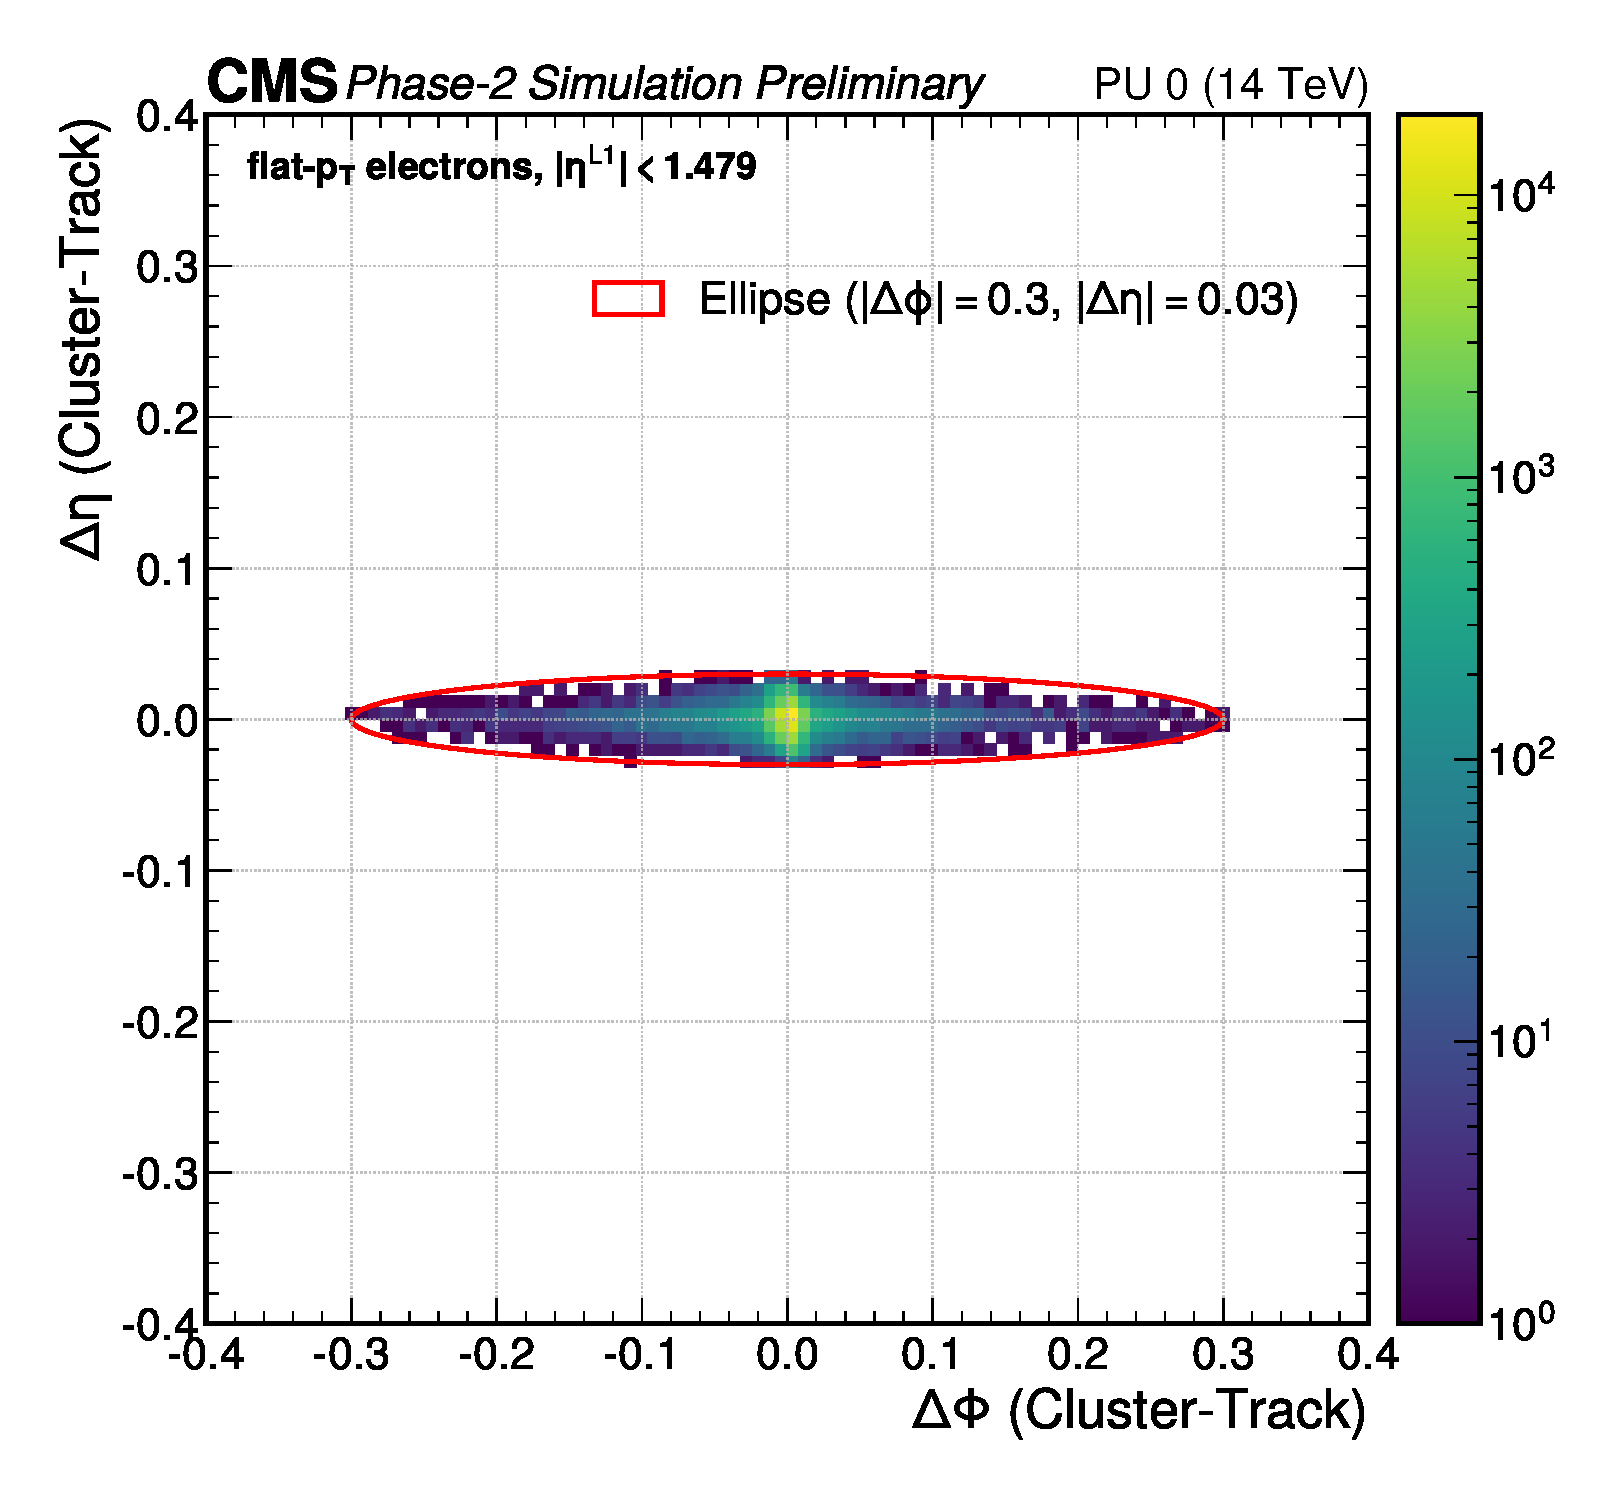
\includegraphics[height=0.42\textheight,trim={0 2cm 0 2.2cm}]{barrel_figs/slides17/etaphi.pdf}
    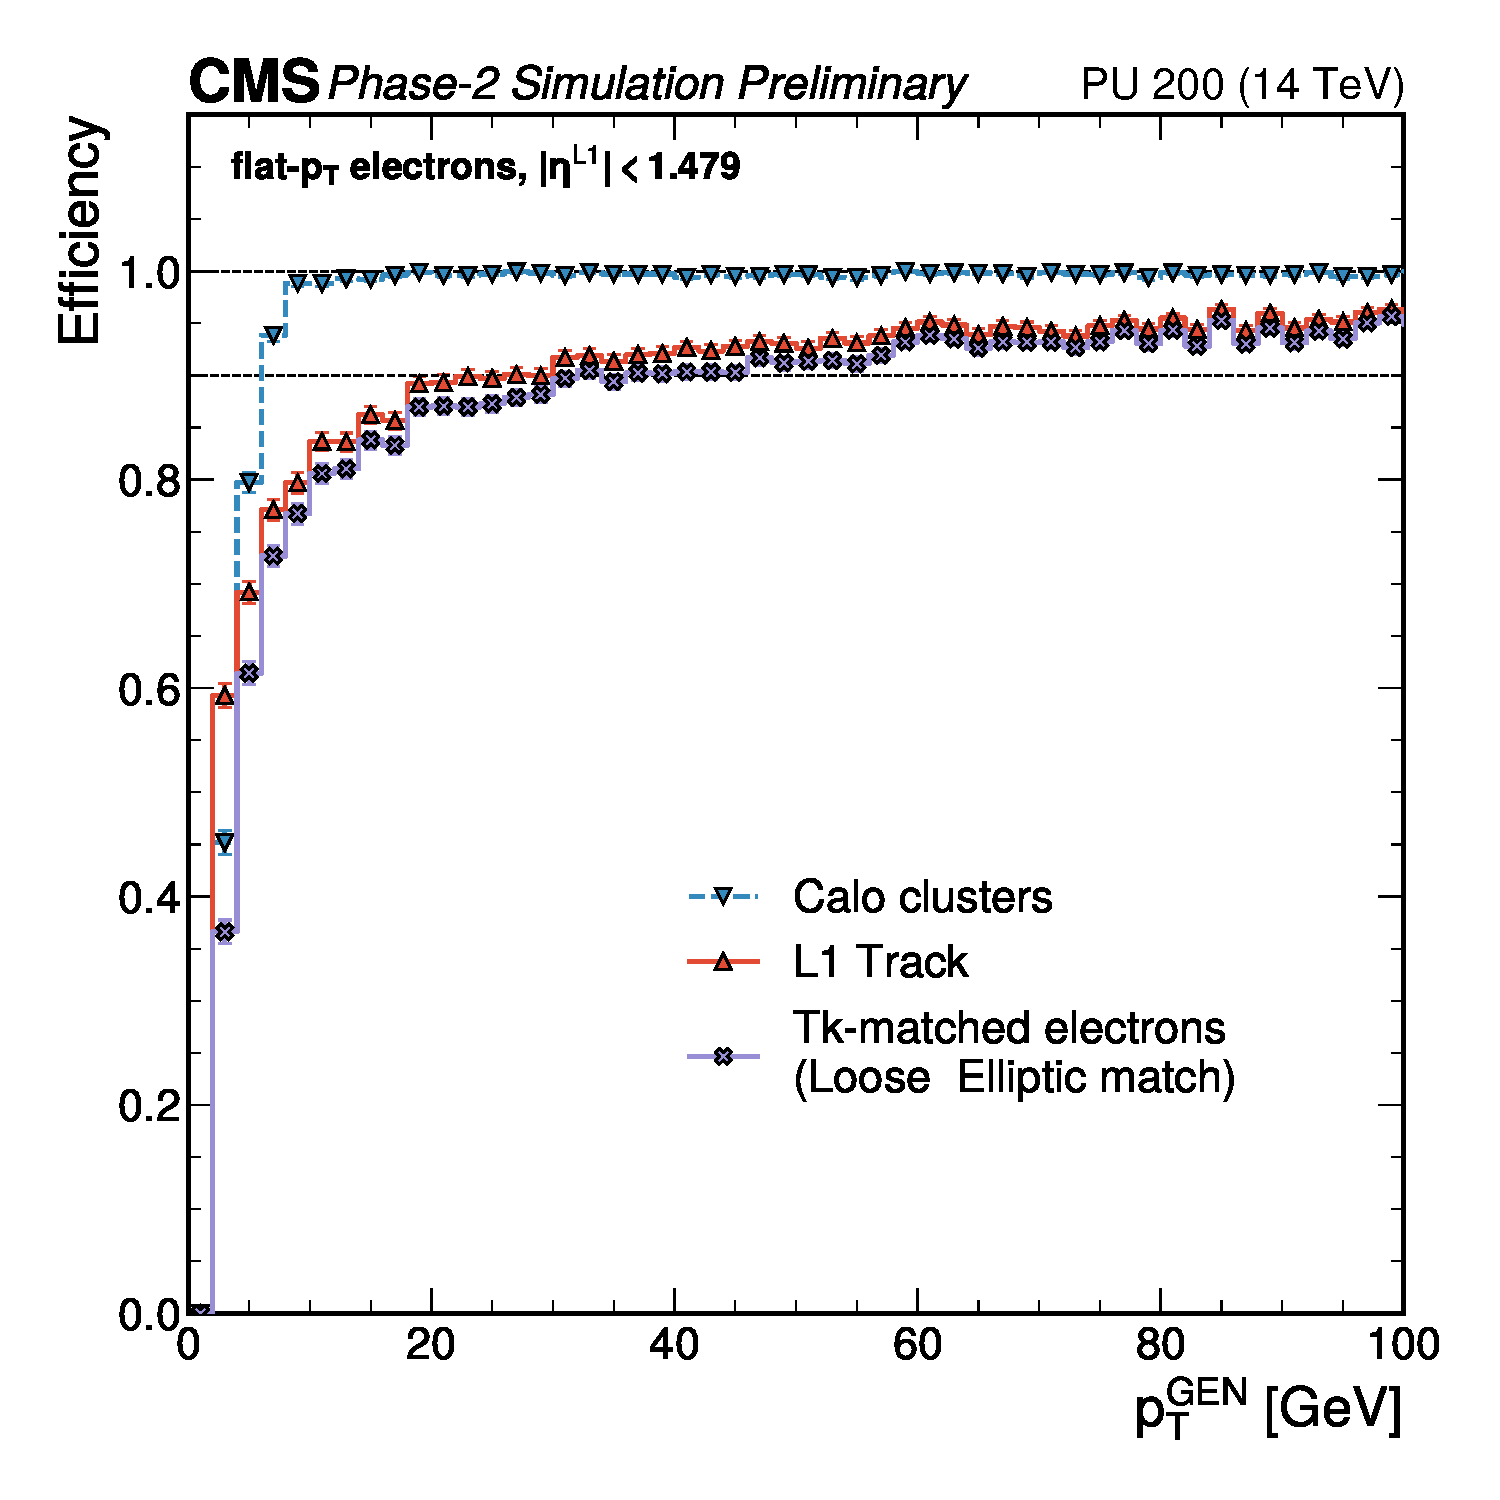
\includegraphics[height=0.42\textheight,trim={0 2cm 0 2.2cm}]{barrel_figs/slides17/pteff.pdf}
\end{figure}

    




\begin{minipage}{\textwidth}
\relscale{0.9}{
Candidate track-calorimeter cluster pairs are selected with a loose elliptic match ($\Delta \phi < 0.3$, $\Delta \eta <0.03$) and no requirements on the track and the cluster.

For training the model, signal candidates are selected based on the geometrical ($\Delta R<0.1$) matching of the cluster with a generated electron particle, while all candidates in a minimum-bias sample are used for the background.



The left plot shows the Track-Cluster $\Delta \eta$ vs $\Delta \phi$ 2D distribution in a 0 PU sample, while the right plot shows the efficiencies of the standalone object, L1 tracks, and Tk-matched candidates as a function of the generated electron $p_{T}$.}
\end{minipage}

\end{frame}











\begin{frame}{Tk-matched Electrons in the barrel: Composite-ID Model}
\begin{columns}[c]

\begin{column}{.666\textwidth}
\begin{figure}
\centering
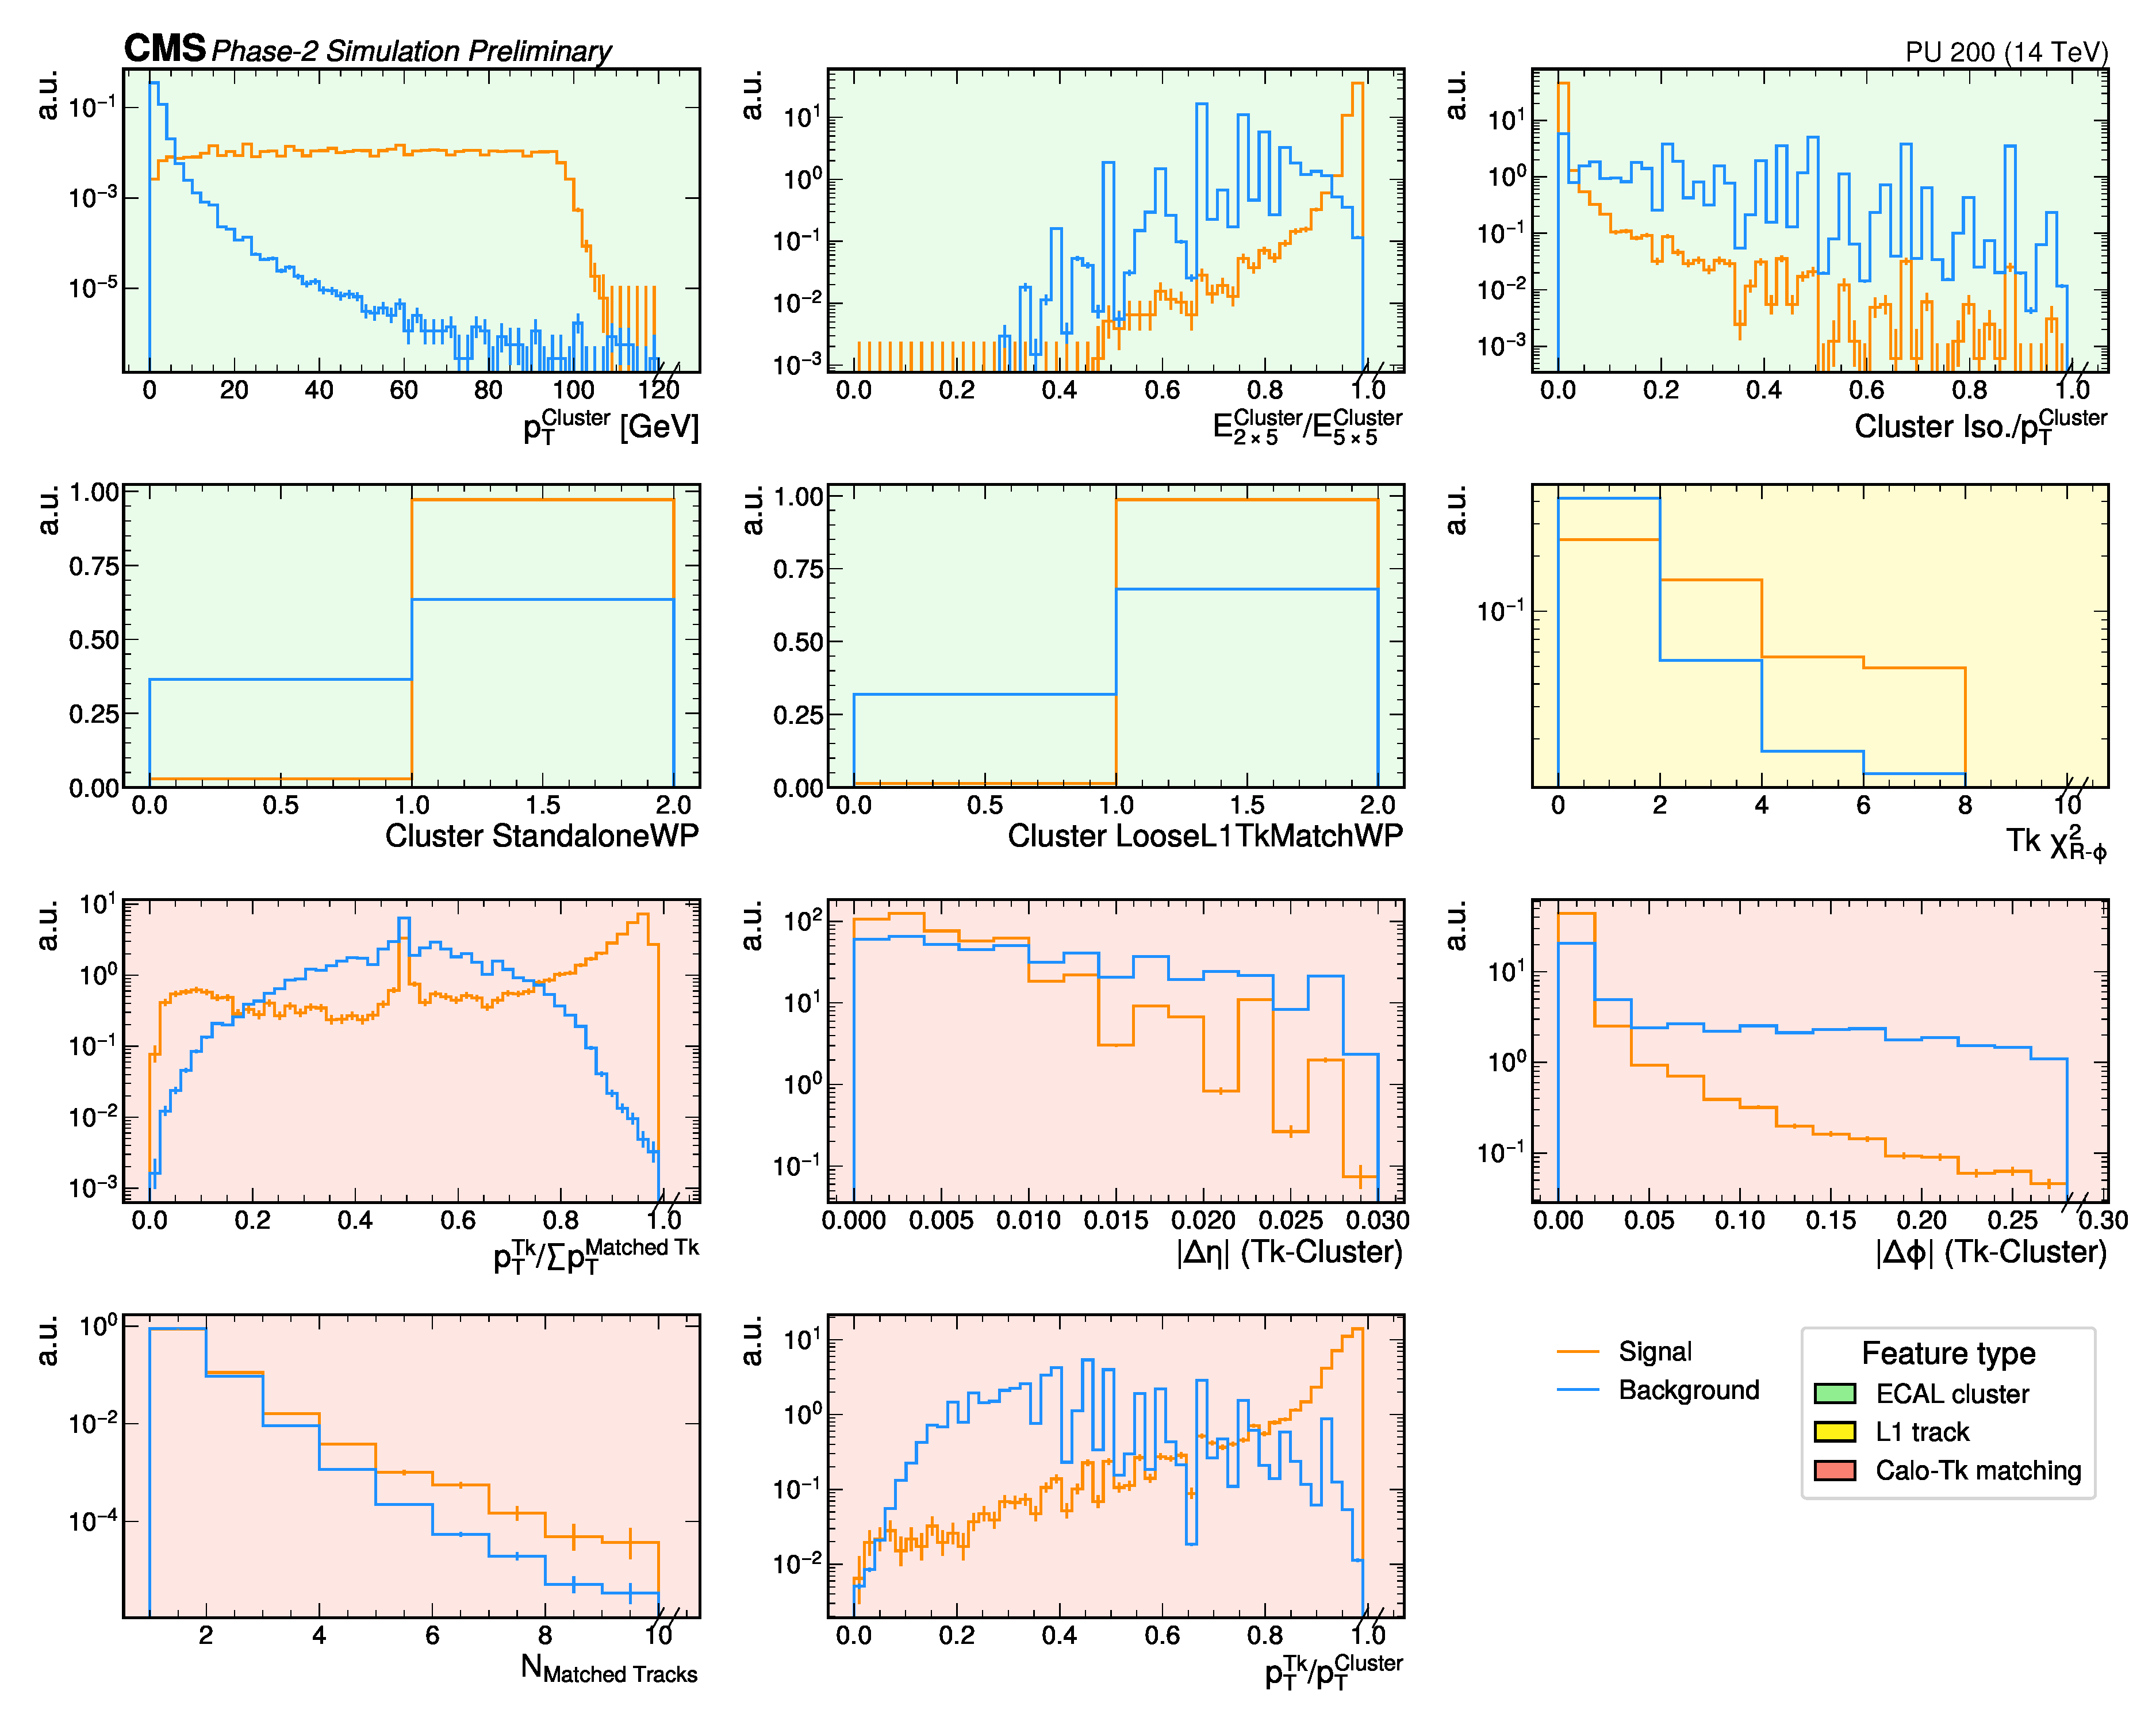
\includegraphics[height=0.8\textheight]{barrel_figs/slides18/features.pdf}
\end{figure}

\end{column}
\begin{column}{.3333\textwidth}
\begin{minipage}{\textwidth}
\relscale{0.666}{
The Composite-ID combines calorimeter cluster shape variables, track qualities, and track-matching features in a single BDT model controlling the identification of track and calorimeter deposit and the tightness of the matching.
\\
The plots show the distributions of the input features for signal and background, \textcolor{blue}{where $E_{2\times5}/E_{5\times5}$ is the ratio of energy in a 2 × 5 to a 5 × 5 ECAL crystal array, Tk $\chi^2_{R-\phi}$ is the track fit $\chi^2$
in the $R-\phi$ plane, while StandaloneWP and LooseL1TkMatchWP are cluster quality flags.}
The signal is defined as track-matched candidates matched to a generated electron in a flat-$p_T$ electrons sample, while all track-matched candidates in a Minimum-bias sample are used for the background.
}
\end{minipage}
\end{column}
\end{columns}

\end{frame}


\begin{frame}{Tk-matched Electrons in the barrel: Composite-ID Model}
\begin{columns}[c]



\begin{column}{.666\textwidth}
\begin{figure}
\centering
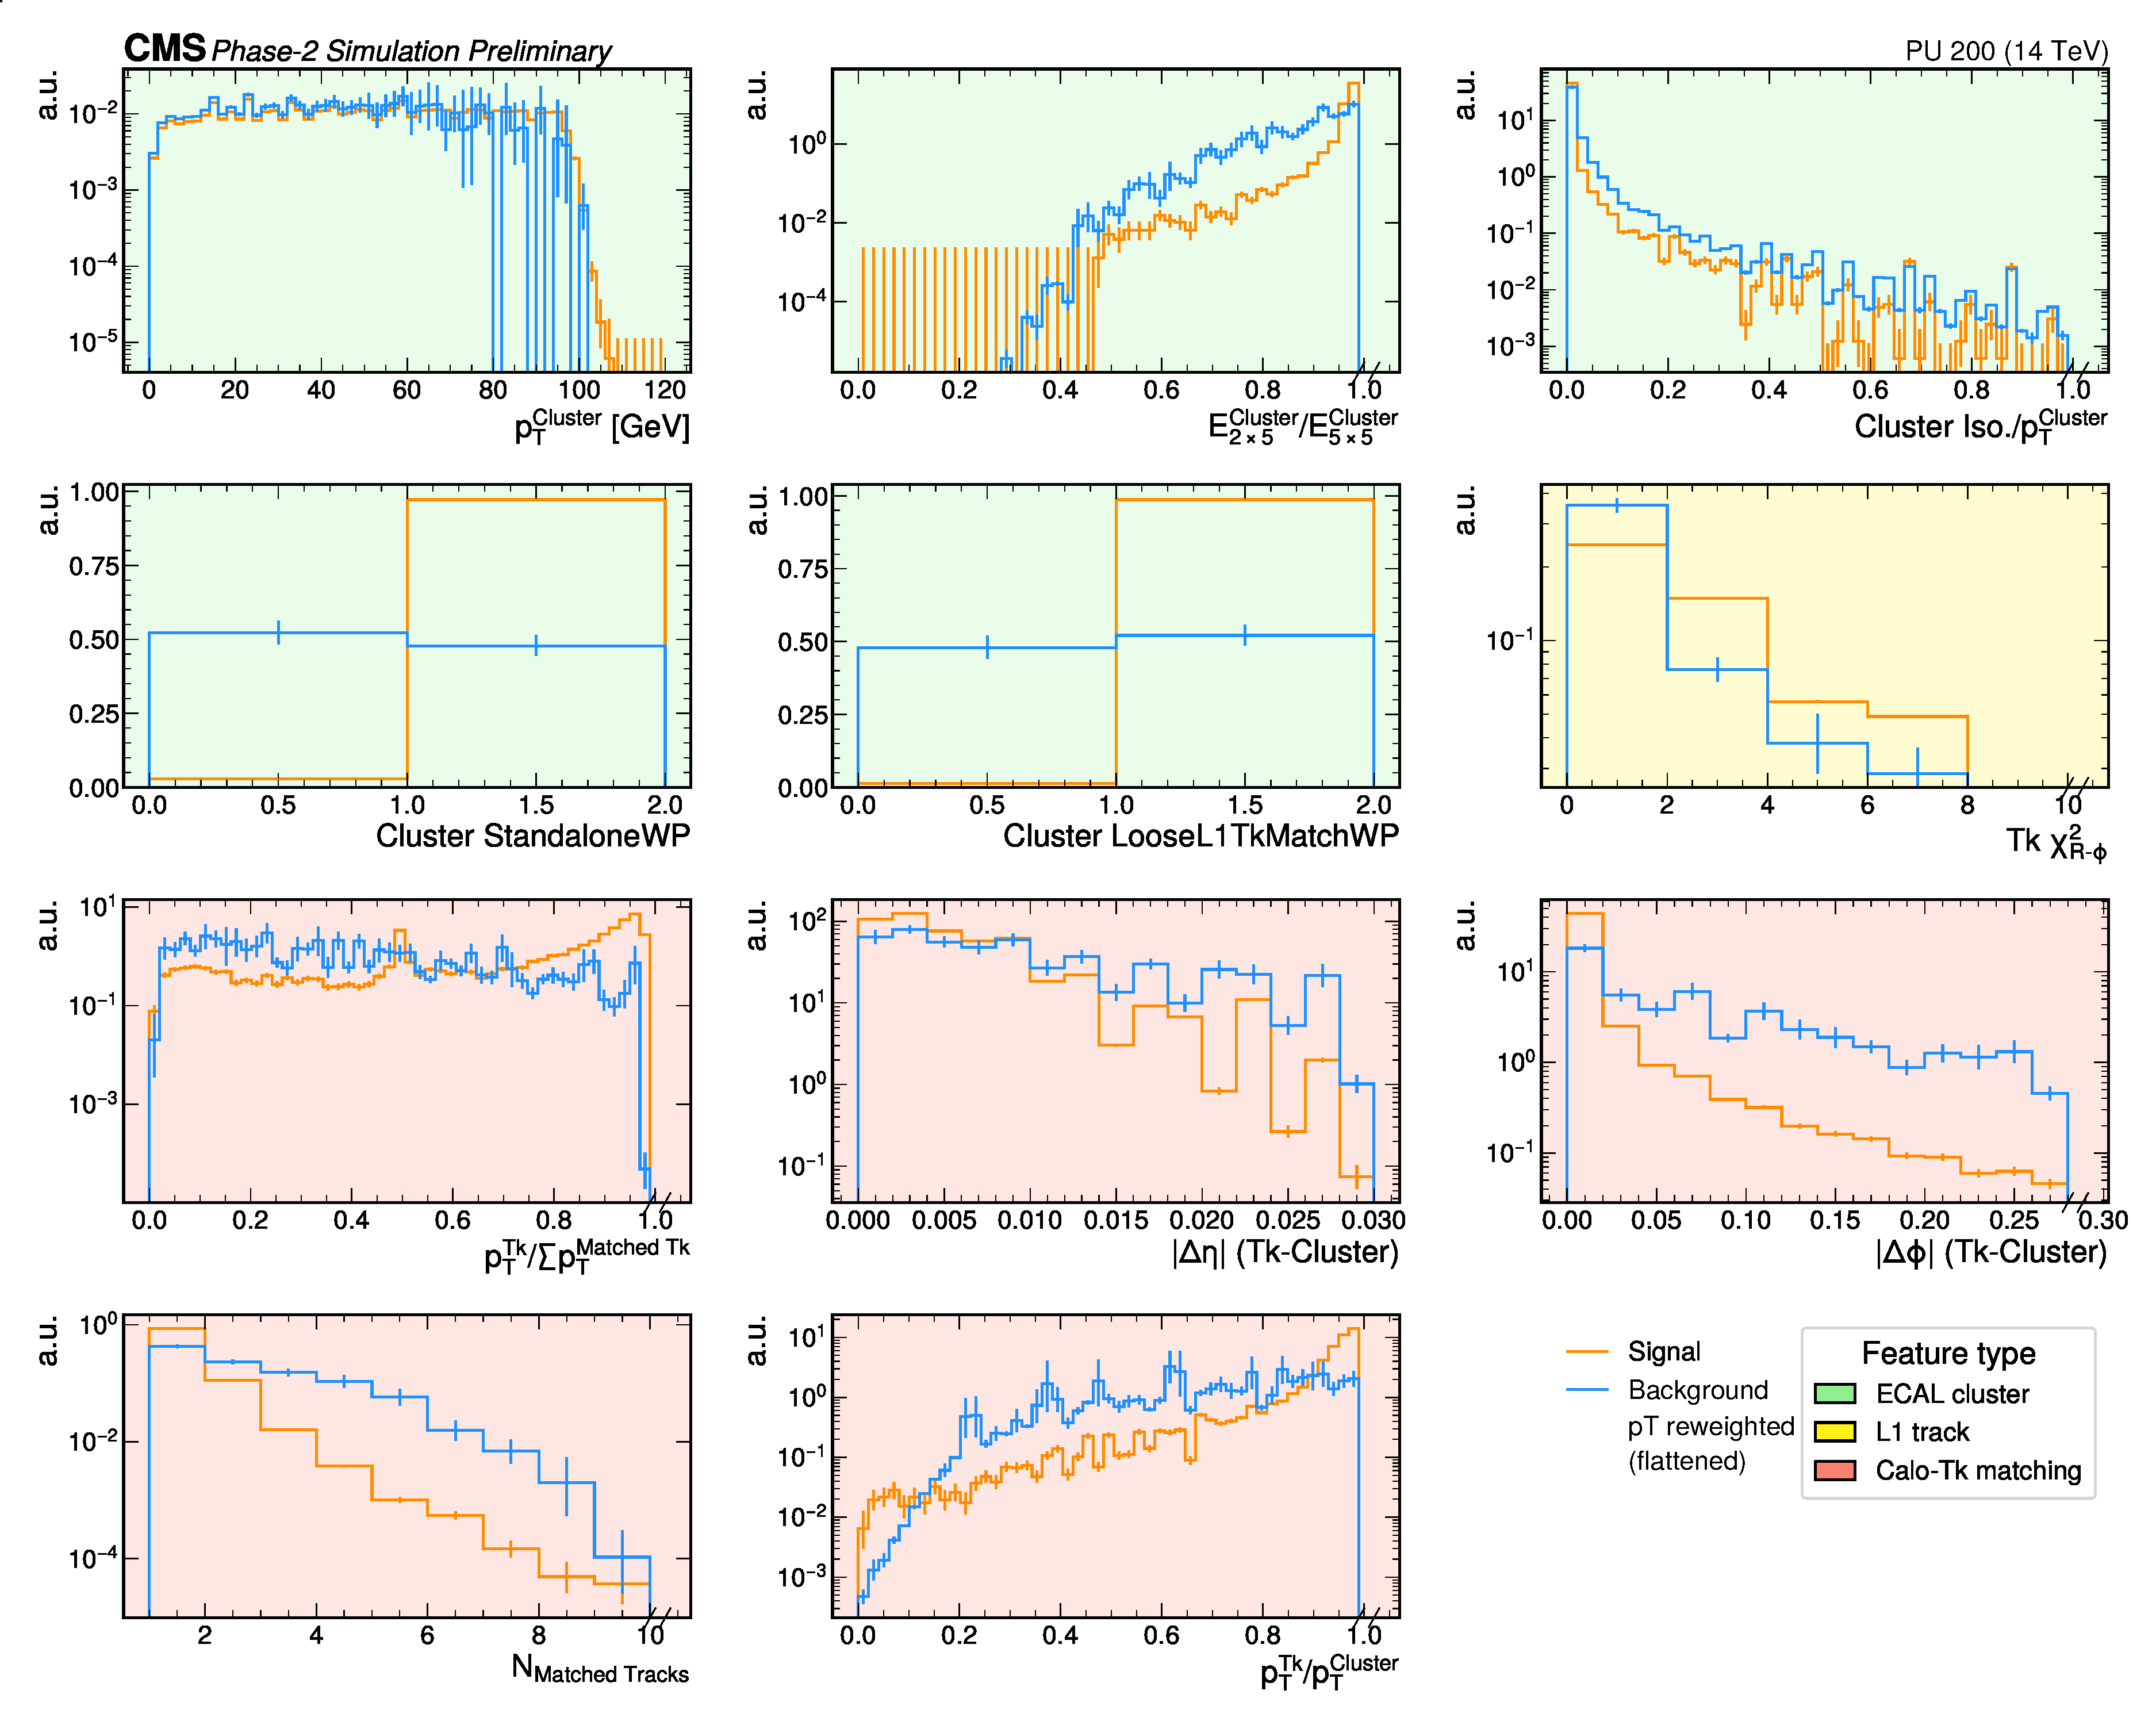
\includegraphics[height=0.8\textheight]{barrel_figs/slides19/features_flat.pdf}
\end{figure}

\end{column}
\begin{column}{.333\textwidth}
\begin{minipage}{\textwidth}
\relscale{0.7}{
To prevent the model from imposing a tight cut on $p_T^{\text{Cluster}}$, the features of all the background candidates used for training were reweighted to flatten the $p_T^{\text{Cluster}}$ distribution (top left plot). 
This improves the efficiency for low-$p_{T}$ electrons.
The plots show the input features of the model after reweighting. 
\\
\\
Unlike the training, the validation is done using the non-reweighted features.
}
\end{minipage}
\end{column}
\end{columns}
\end{frame}



\begin{frame}{Tk-matched Electrons in the barrel: Composite-ID Model}

\begin{columns}[c]

\begin{column}{.45\textwidth}
\begin{minipage}{\textwidth}

The BDT scores for signal and background are obtained from the bit-wise emulator implemented using Conifer with \texttt{ap\_fixed} precision.
The plot on the right shows the receiver operating characteristic curve (ROC) curve of the BDT model \textcolor{blue}{and the area under the curve (AUC)} using the bit-wise firmware emulator in different bins of $p_T^{\text{Cluster}}$.
\end{minipage}
\end{column}

\begin{column}{.5\textwidth}
\vspace{-1.5cm}
\begin{figure}
\centering
    \vspace{0.5cm}
    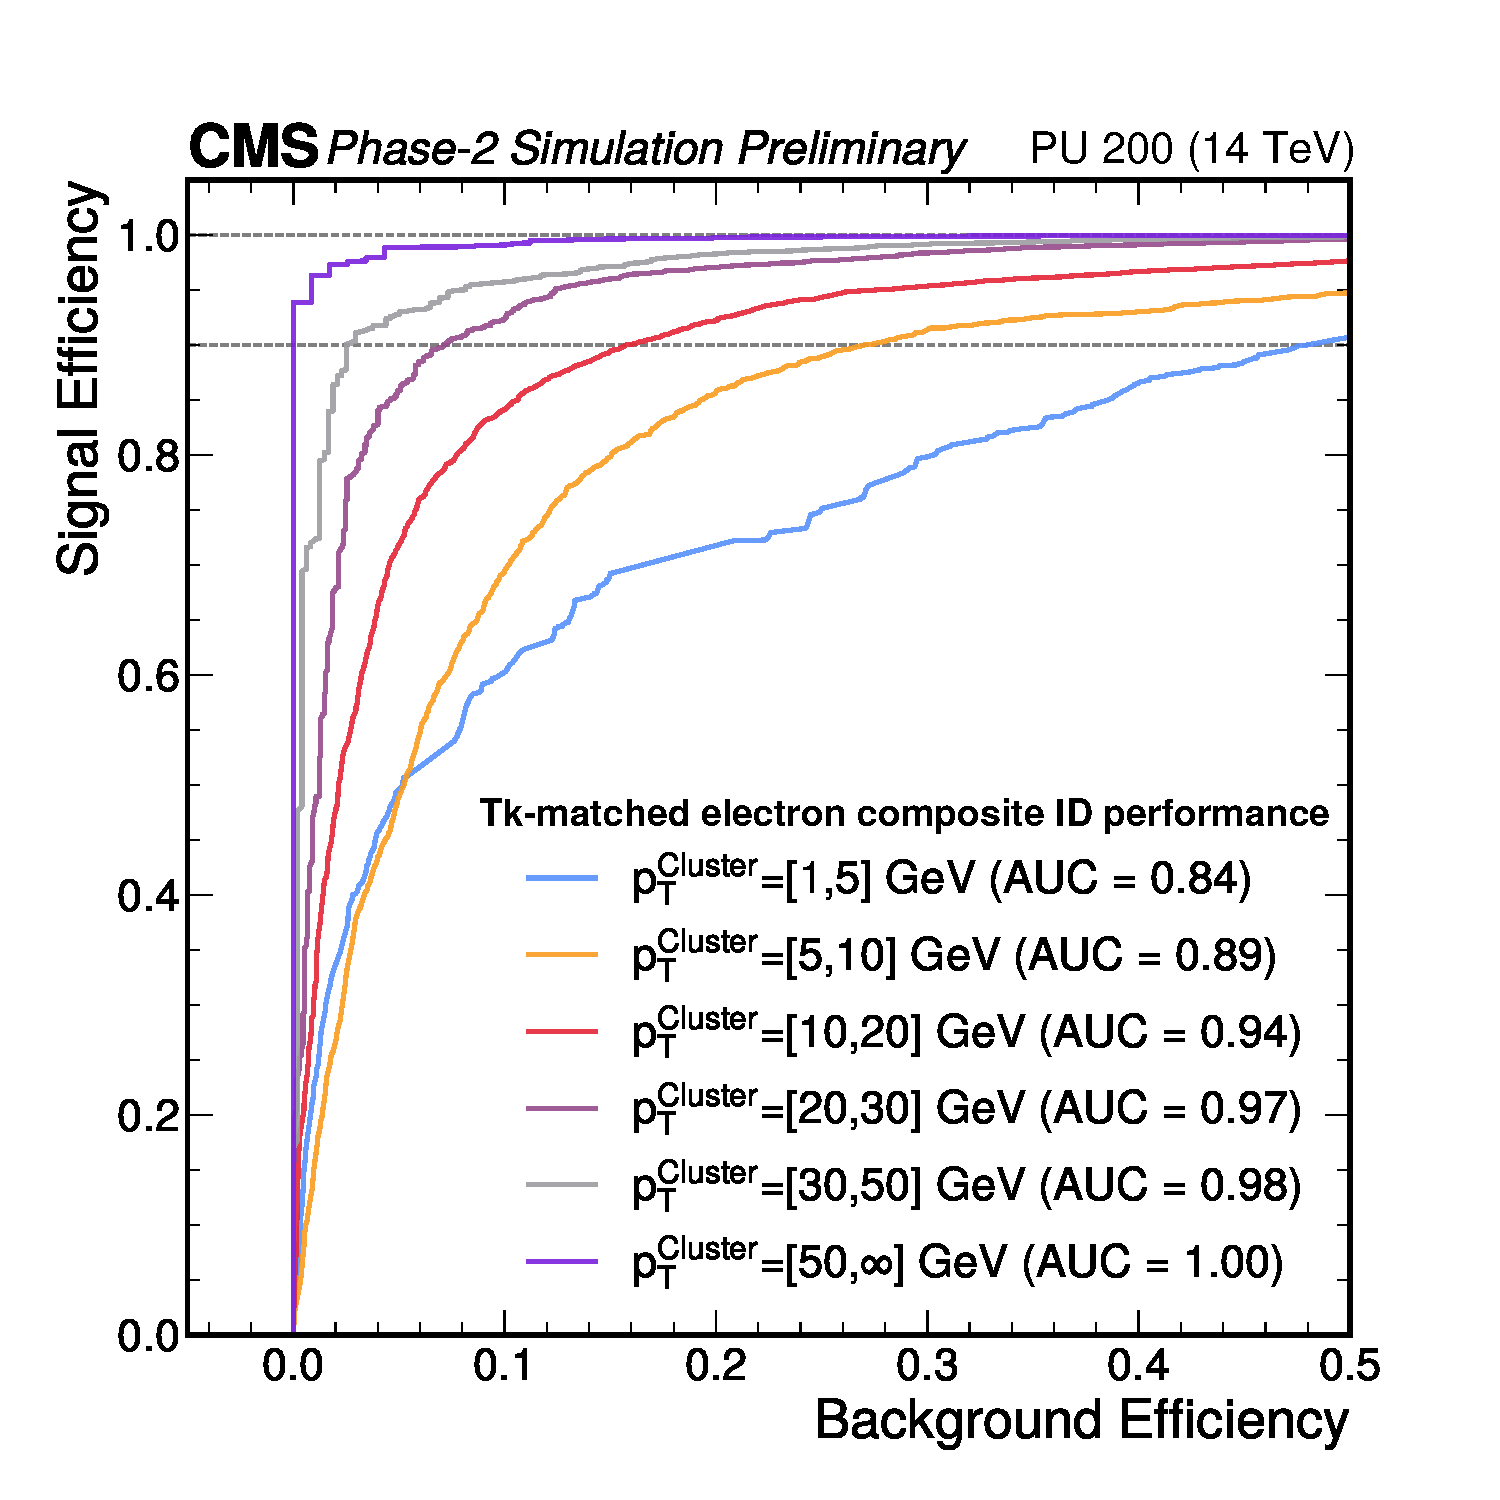
\includegraphics[width=\textwidth]{barrel_figs/DPS_pt_roc-1.pdf}
\end{figure}
\end{column}

\end{columns}
\end{frame}



\begin{frame}{Tk-matched Electrons in the barrel: Elliptic vs Composite ID performance}
\begin{figure}
\centering
    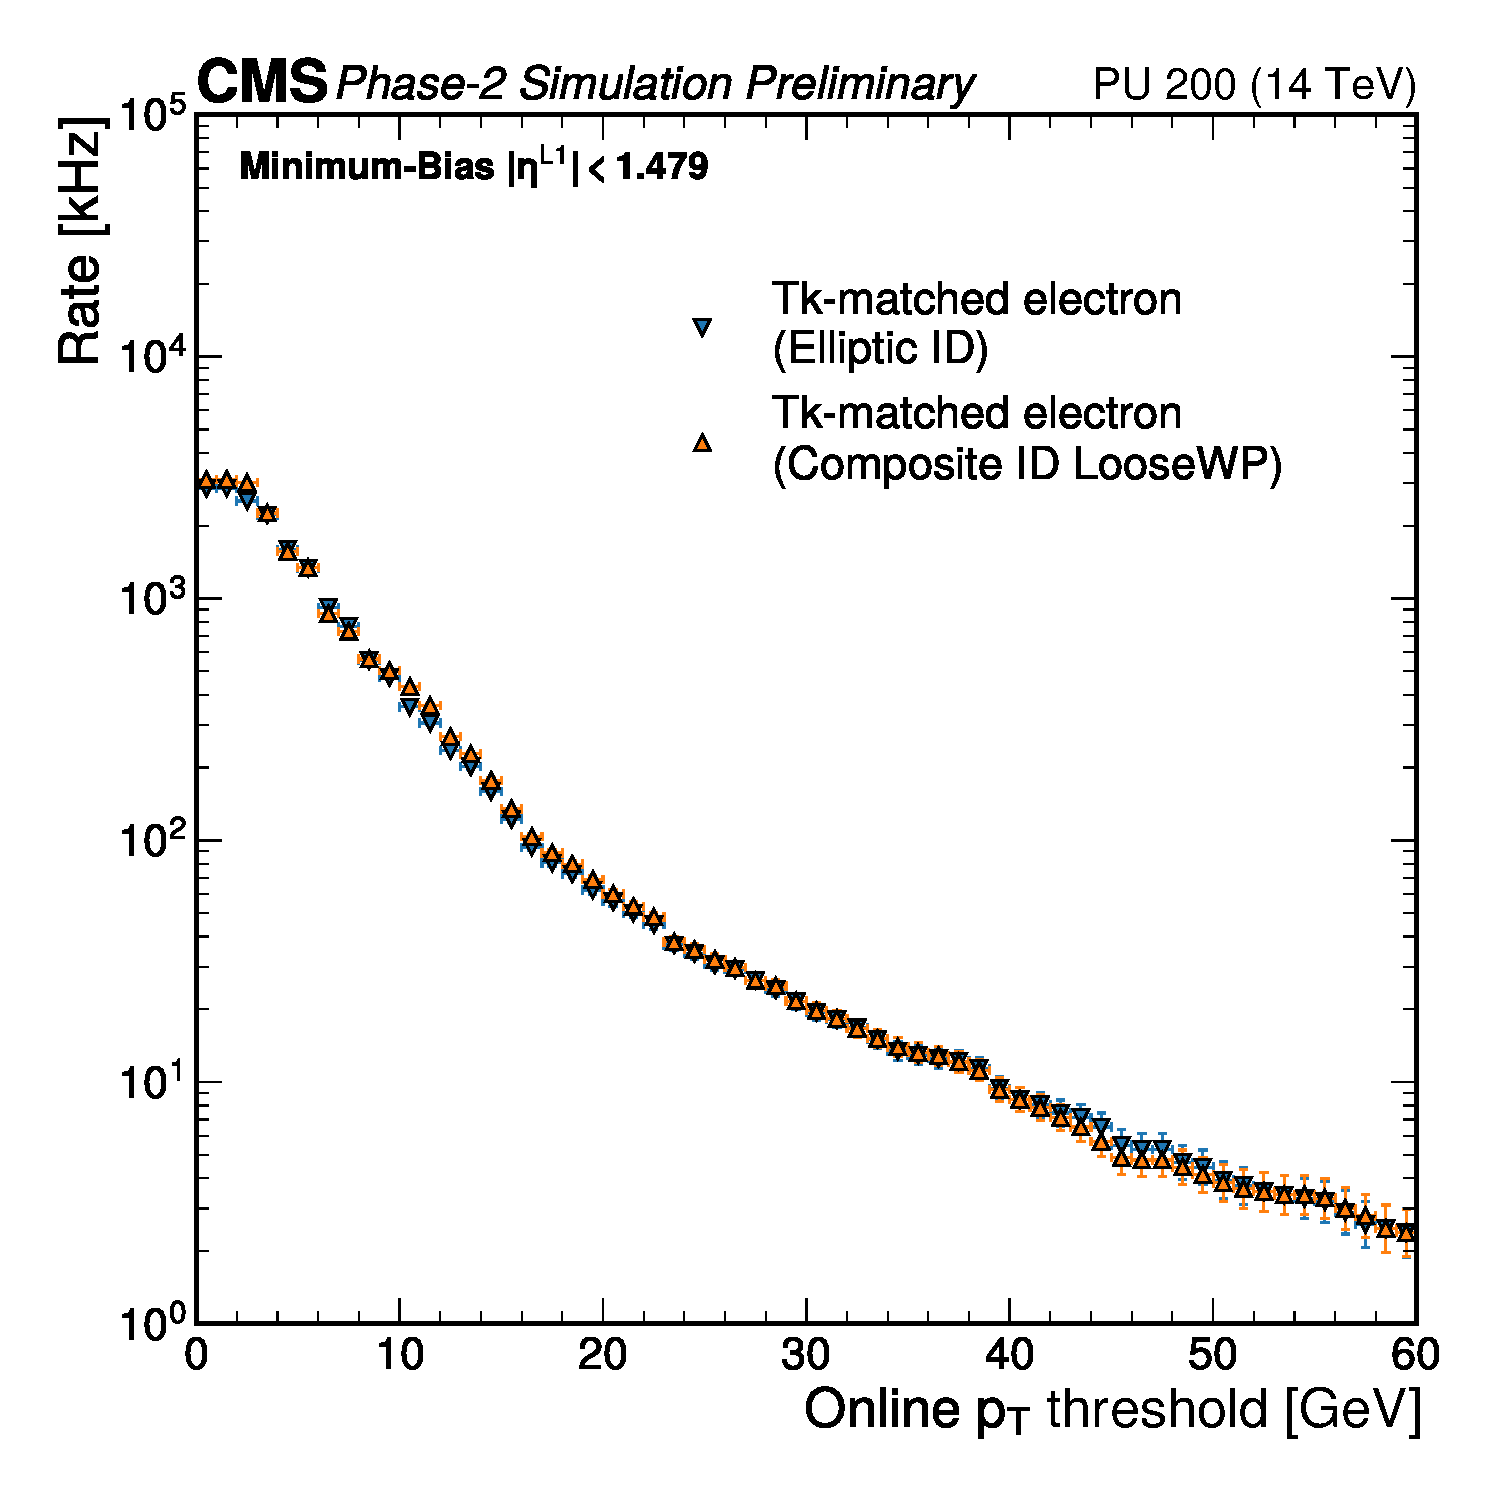
\includegraphics[height=0.475\textheight,trim={0 2cm 0 2.2cm}]{barrel_figs/slides21/rate.pdf}
    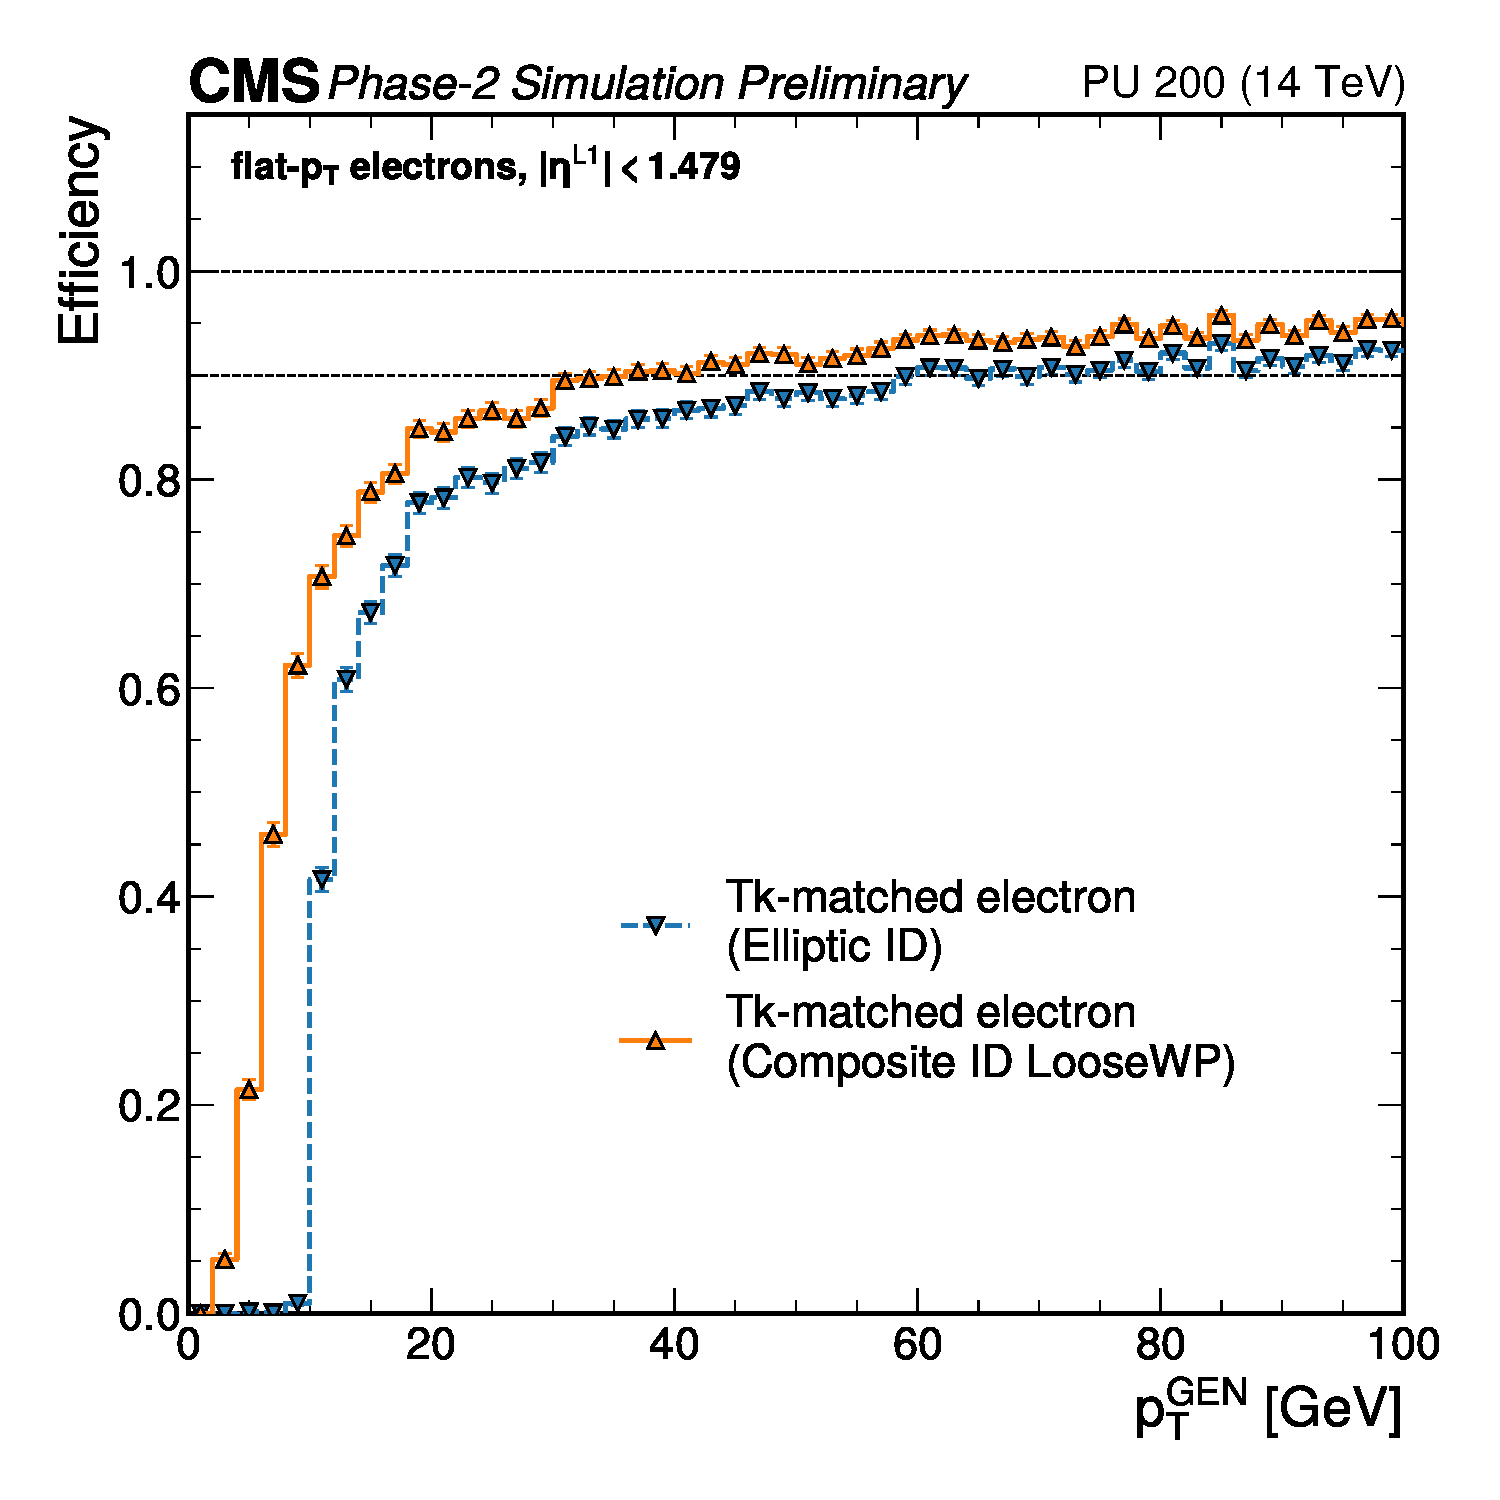
\includegraphics[height=0.475\textheight,trim={0 2cm 0 2.2cm}]{barrel_figs/slides21/pteff.pdf}

\end{figure}
\begin{minipage}{\textwidth}
\relscale{0.7}{
To compare the Composite-ID with the Elliptic-ID, two working points (WPs) applied in different $p_T$ bins were created: a tight WP that matches the efficiency of the Elliptic-ID and a loose WP that matches the rate of the elliptic-ID.

The left plot compares the rate as a function of the cluster $p_T$, while the right plot shows the efficiency as a function of the $p^{\text{Gen}}_{T}$. The new Composite-ID model allows for a substantial efficiency gain compared to the elliptic-ID at parity of rate (Loose WP), especially in the low $p_T$ region.
This is very beneficial for the typical Double Electron seed of the baseline Menu, which has a threshold of 25, 12 GeV.
}
\end{minipage}
\end{frame}


\begin{frame}{Tk-matched Electrons in the barrel: Elliptic vs Composite ID performance}
\begin{figure}
\centering
    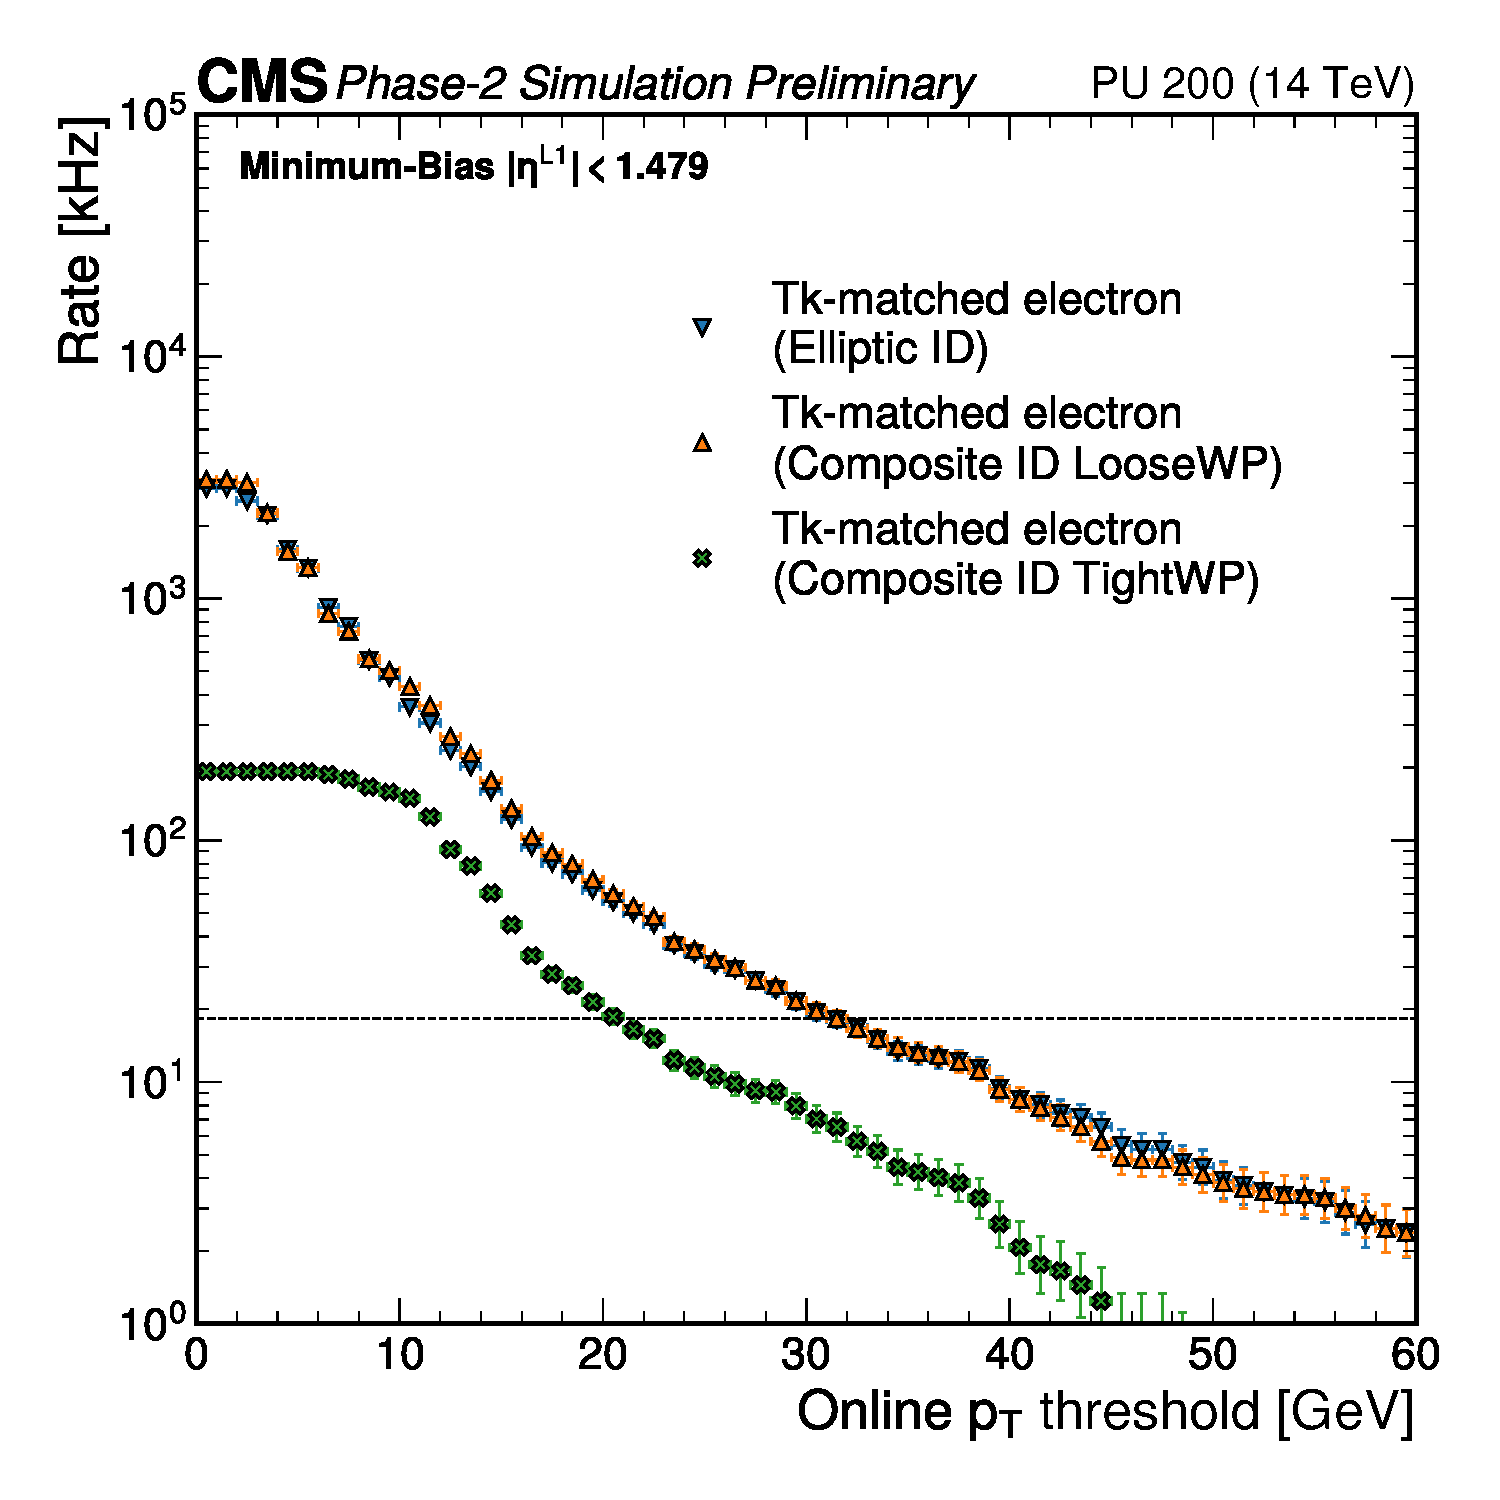
\includegraphics[height=0.55\textheight,trim={0 2cm 0 2.2cm}]{barrel_figs/slides22/rate.pdf}
    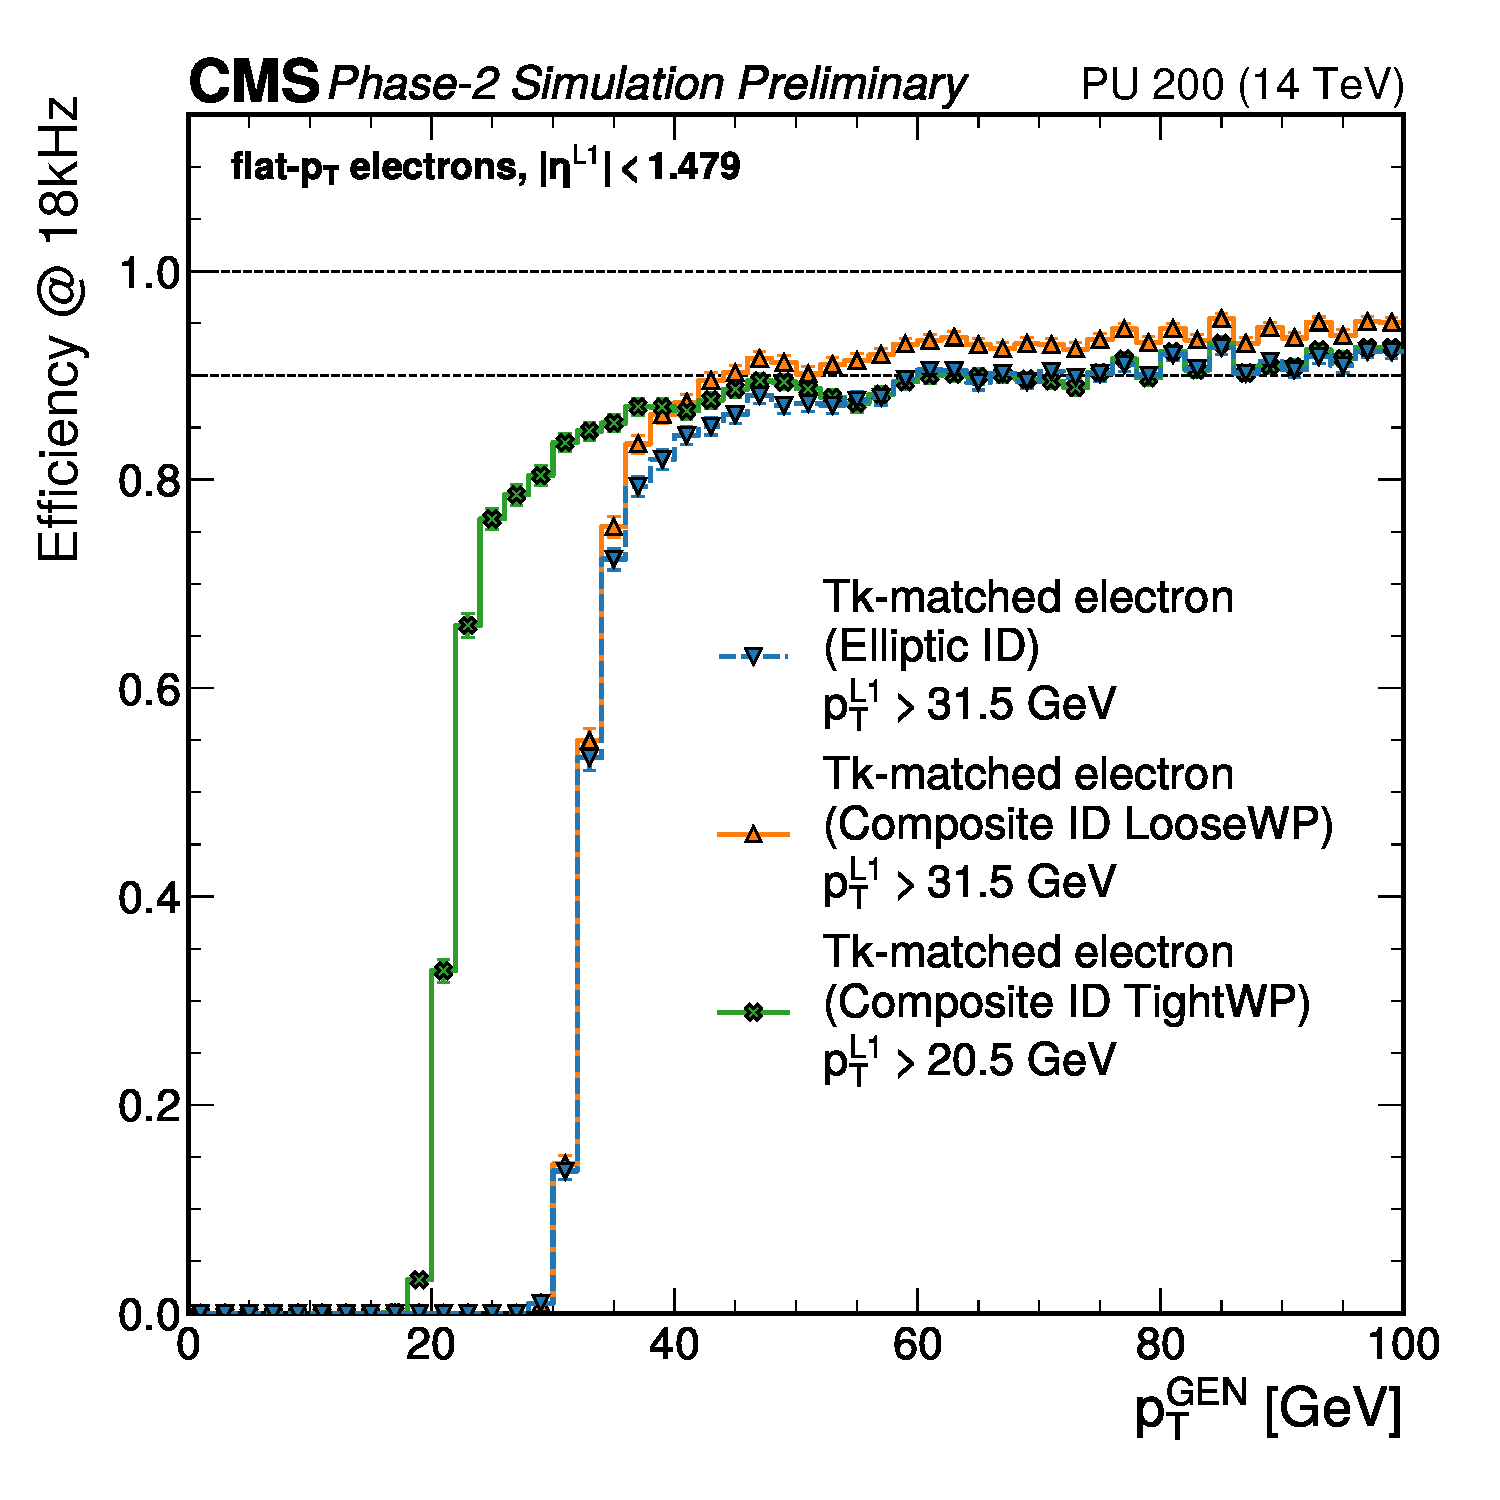
\includegraphics[height=0.55\textheight,trim={0 2cm 0 2.2cm}]{barrel_figs/slides22/pteff-1.pdf}

\end{figure}
\begin{minipage}{\textwidth}
\relscale{0.8}{
Single lepton trigger performance using the Elliptic-ID and the Composite-ID with different working points.
The left plot illustrates the rate as a function of the cluster $p_T$. The right plot compares the efficiency as a function of the $p_{T}$ of the generated electron for a fixed 18 kHz rate, corresponding to the barrel bandwidth for Run-3 like thresholds. 
}
\end{minipage}
\end{frame}


\begin{frame}{Tk-matched Electrons in the barrel: Composite-ID firmware emulation}

\begin{columns}[c]

\begin{column}{.6\textwidth}


\begin{minipage}{\textwidth}


\relscale{0.6}{

The model has been synthesized in firmware using the Conifer~\cite{conifer} library and Vivado HLS.
The input features are quantized using the \texttt{ap\_fixed} format with nine bits for the integer and fifteen bits for the decimal precision, while the raw scores are quantized using 4 and 12 bits for the integer and decimal parts, respectively.
The model is synthesized for a frequency of 180MHz, matching the implementation of the egamma reconstruction in the Correlator Layer-1 boards.
The table illustrates the estimated resource utilization on a Xilinx Virtex UltraScale+ VU13P FPGA.
The plot on the right shows the ROC curves for the XGBoost \cite{xgb} model and the quantized model emulated with Conifer.\\
\\

}
\begin{center}
\resizebox{0.75\textwidth}{!}
{
\centering
\begin{tabular}{rccccc}
\hline
\centering
  & BRAM & DSP & FF & LUT \\
\hline
SLR& 0.0\%& 0.0\% & 0.12\% & 6.5\% \\
Total & 0.0\%& 0.0\% & 0.02\% & 1.6\%   \\
\hline
\end{tabular}
}

\begin{table}
\resizebox{0.75\textwidth}{!}{%
\begin{tabular}{ccc}
\hline
&Clock cycles & Latency \\
\hline
Clock (5.56 ns) &5 & 27.8 ns\\
\hline
\end{tabular}
}
\end{table}
\end{center}

\end{minipage}
\end{column}

\begin{column}{.4\textwidth}
\begin{figure}
\centering
    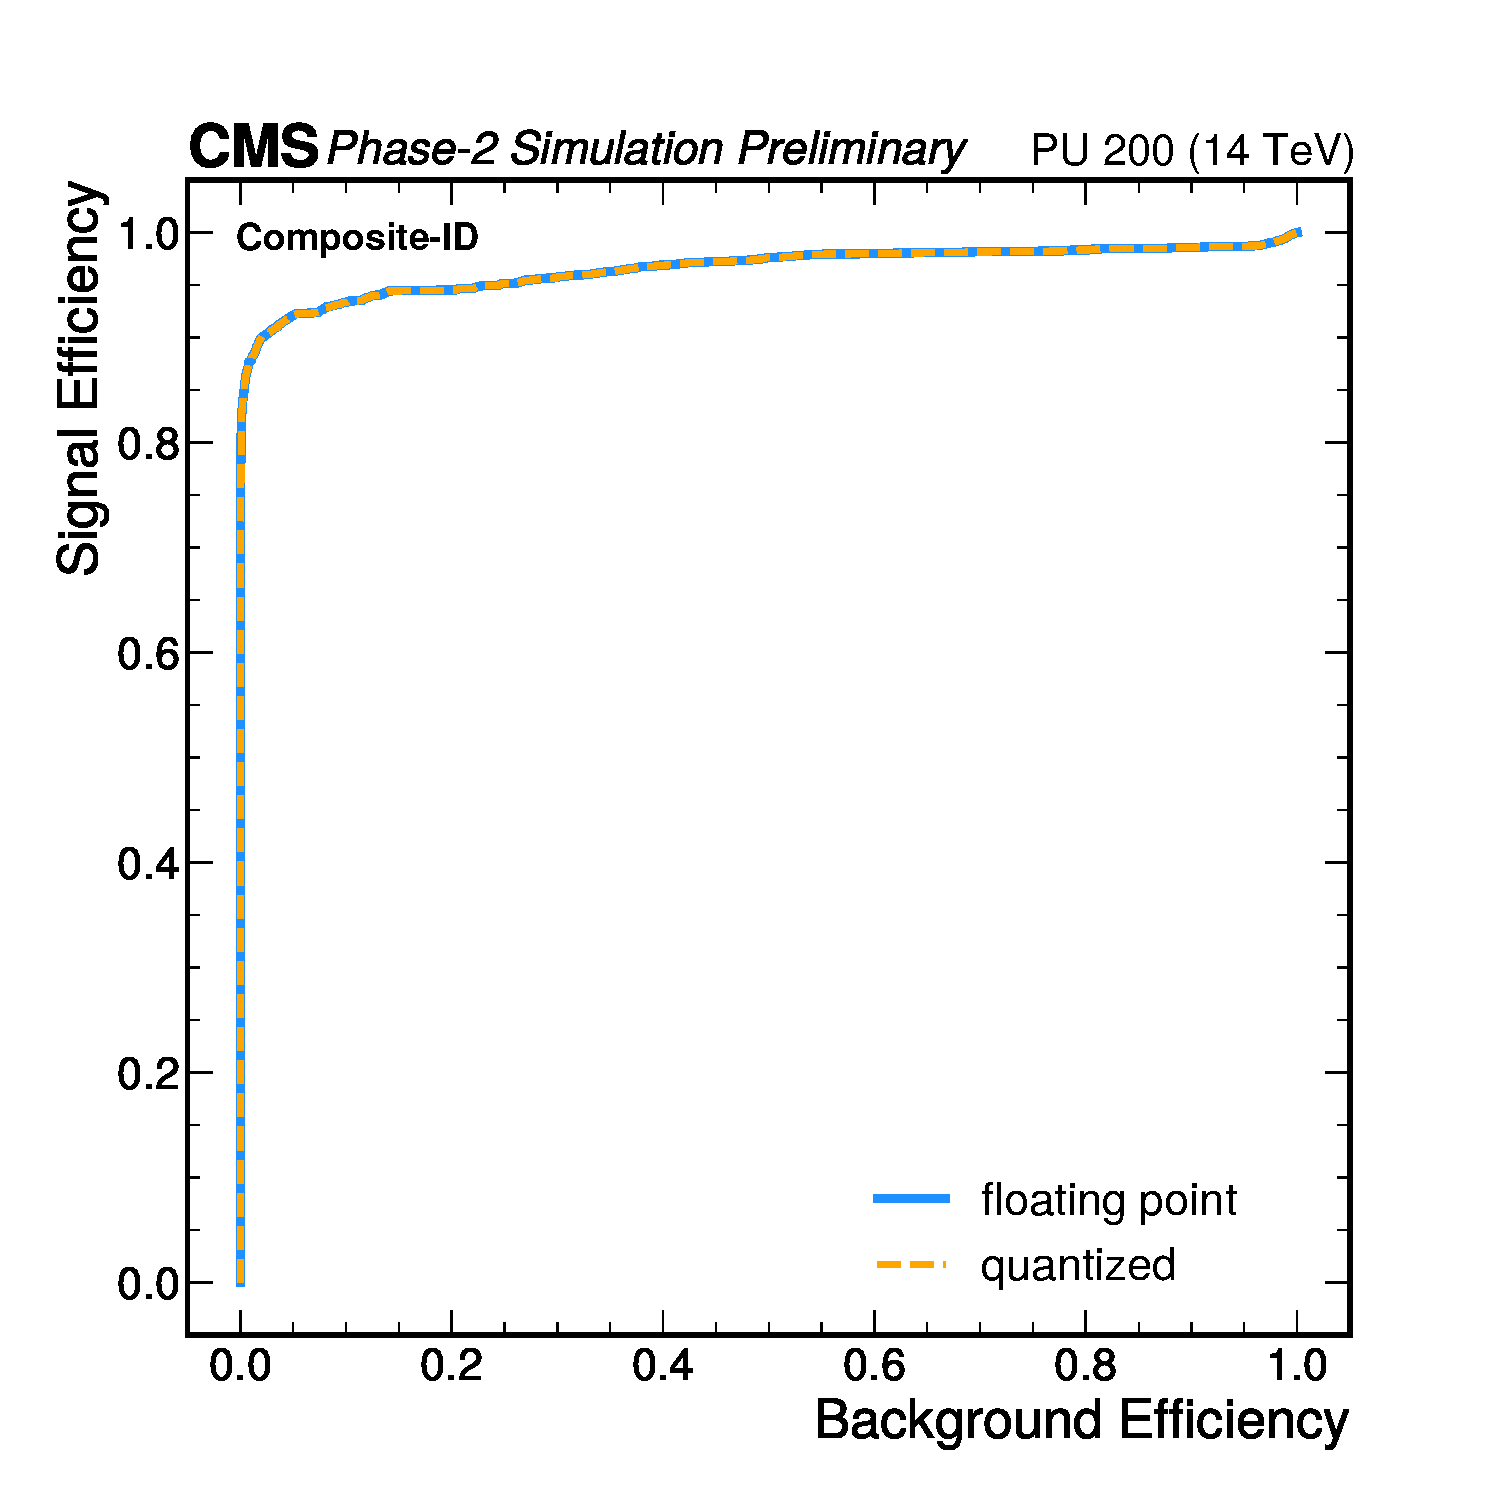
\includegraphics[width=\textwidth]{barrel_figs/rocs.pdf}
\end{figure}


\end{column}

\end{columns}
\end{frame}












\section{References}



\begin{frame}{References}
\begin{thebibliography}{99}
\bibitem{tdr-p2-l1} CMS Collaboration , "The Phase-2 Upgrade of the CMS Level-1 Trigger", \emph{CERN-LHCC-2020-004}
\url{https://cds.cern.ch/record/2714892?ln=en}.
\bibitem{tdr-p2-l1-eg} CMS Collaboration , "Electron Reconstruction and Identification in the CMS Phase-2 Level-1 Trigger", \emph{CERN-CMS-DP-2023-047}
\url{https://cds.cern.ch/record/2868782?ln=en}.
\bibitem{conifer} Conifer, \url{https://github.com/thesps/conifer}.
\bibitem{xgb} XGBoost, \url{https://xgboost.readthedocs.io/en/stable/}.



\end{thebibliography}


\end{frame}


\end{document}
